%% The following is a directive for TeXShop to indicate the main file
%%!TEX root = diss.tex

\chapter{Interpretation of 3D Reconstruction Model}
\label{ch:3DRecon_Interp}
In order to validate the 3D reconstruction mapping derived from the Chapter~\ref{ch:3DRecon_Mapping}, evaluation of the object centric model into appropriate solutions must be shown. Our interpreter is based on the direct evaluation of the performance of each 3D reconstruction algorithm under different conditions presented in Chapter~\ref{ch:3DRecon_Mapping}. From this analysis of how algorithms perform on objects which have different visual and geometric properties, an algorithm(s) can be definitively chosen based on which performed best on the training images.

% The three algorithms introduced in our test bench are: the PMVS proposed by \citeauthor{furukawa2010accurate}, the example-based Photometric Stereo proposed by \citeauthor{hertzmann2005example}, and a standard gray-coded Structured Light technique with error rejection.

Although only three algorithms selected, all of which are the top performers in the corresponding field, and are sufficient to demonstrate the framework's ability to translate the descriptive model into a reconstruction. Furthermore, the integration of a new algorithm requires the same process preseneted in Chapter~\ref{ch:3DRecon_Mapping}, allowing researchers to contribute novel algorithms to the framework.

\section{Parameter settings}
The first step of the process is to estimate the amount of property in the object. We use a try-and-fit approach, where the user use an . A similar approach can be found in the~\cite{Berkiten:2016:ARB}, and 

\begin{figure}[h!]
\centering
\begin{tabular}{cc}
  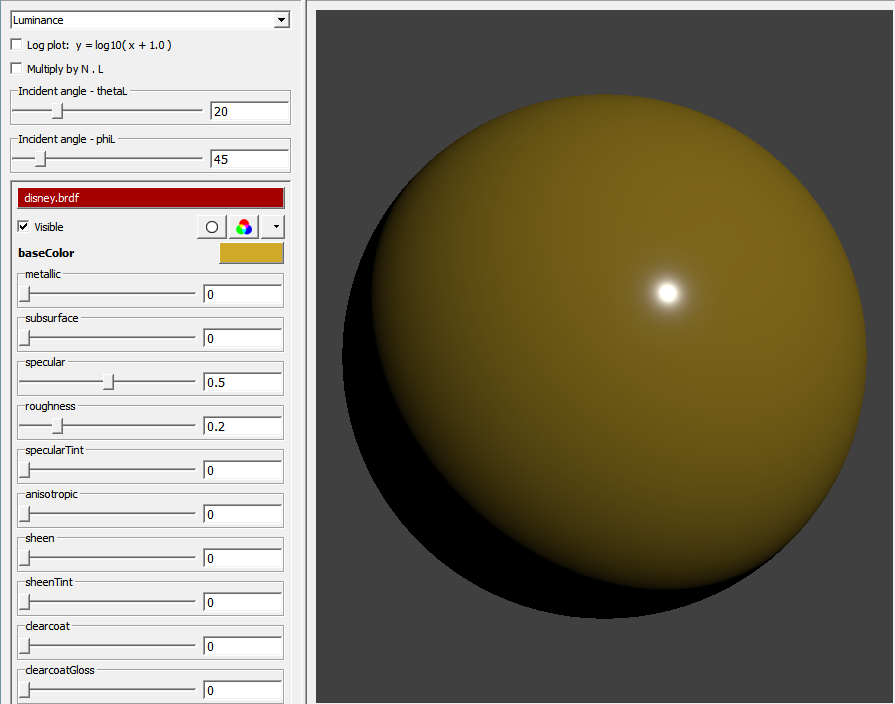
\includegraphics[width=0.5\textwidth]{interp/ui_sphere.PNG}&
  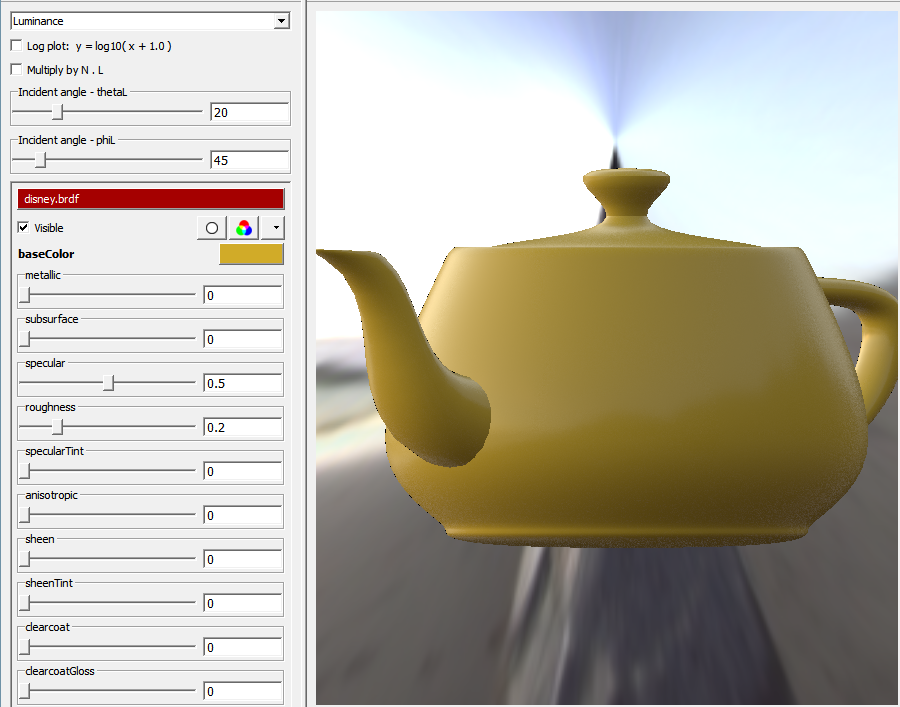
\includegraphics[width=0.5\textwidth]{interp/ui_teapot.PNG}\\
  (a) Lit sphere & (b) Lit teapot\\
\end{tabular}
\caption{The UI of determining the albedo, specular, and roughness of the surface. The albedo is set as around 0.8, which is determined by the value channel of HSV colour. The specular and roughness is set as 0.5, 0.2, respectively. (a) demonstrates the effect of the property setting on a sphere while (b) on a teapot.}
\label{fig:ui}
\end{figure}

\section{Synthetic Datasets}
We use one object shown in Figure~\ref{fig:synth_data}, and four property settings in Table~\ref{tab:prop_list_synth_data} to test the validity of the abstraction. Those four settings represents four classes of objects discussed in Chapter~\ref{ch:3DRecon_Desc}. The best suited algorithm as suggested by the mapping derived from Chapter~\ref{ch:3DRecon_Mapping} is included.
\begin{table}[h]
  \centering
  \begin{tabular}{l*{5}{c}}
  \hline
  \textbf{Property} & Texture & Albedo & Specular & Roughness & Best-suited techniques\\
  \hline
  (a) & 0.2 & 0.8 & 0.2 & 0.8 & PS, SL\\
  (b) & 0.2 & 0.8 & 0.5 & 0.2 & PS, SL\\
  (c) & 0.8 & 0.8 & 0.2 & 0.8 & MVS, PS, SL\\
  (d) & 0.8 & 0.8 & 0.5 & 0.2 & MVS, PS, SL\\
  \hline
  \end{tabular}
  \caption{Property lists of the test objects.}
  \label{tab:prop_list_synth_data}
\end{table}

\begin{figure}[h!]
\centering
\begin{tabular}{cc}
  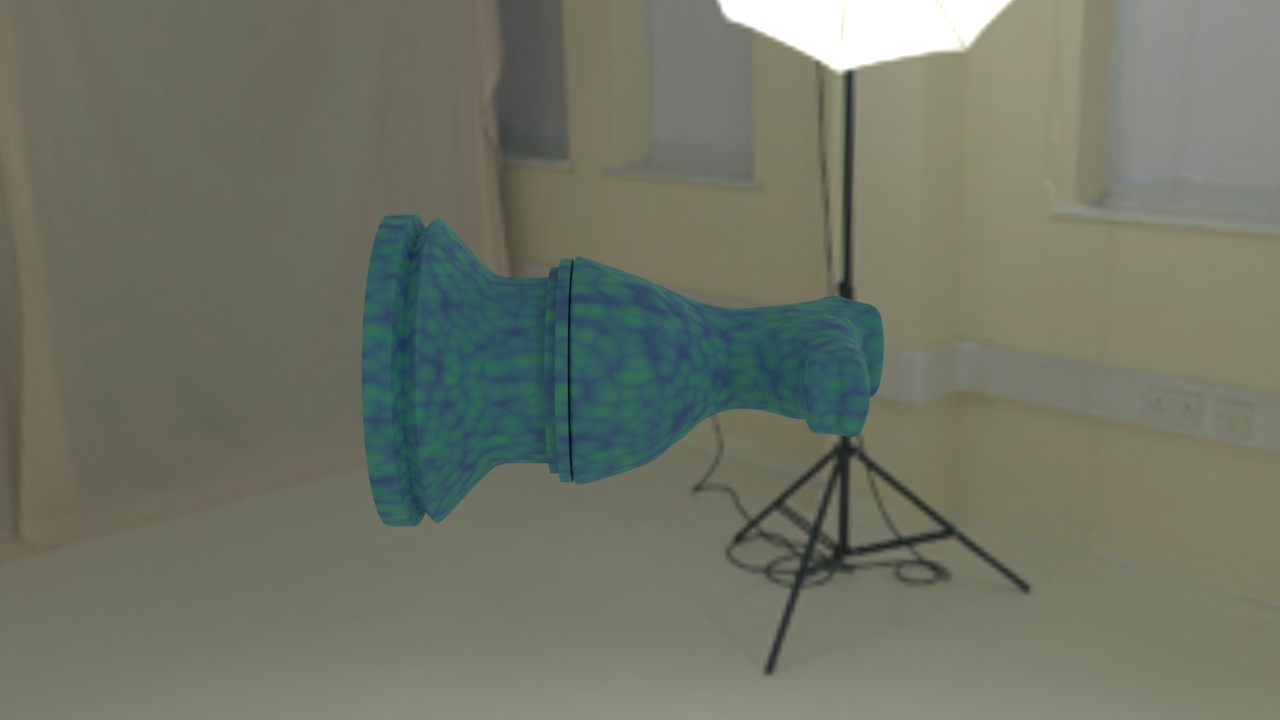
\includegraphics[width=0.33\textwidth]{interp/synth_data/knight/knight_mvs}&
  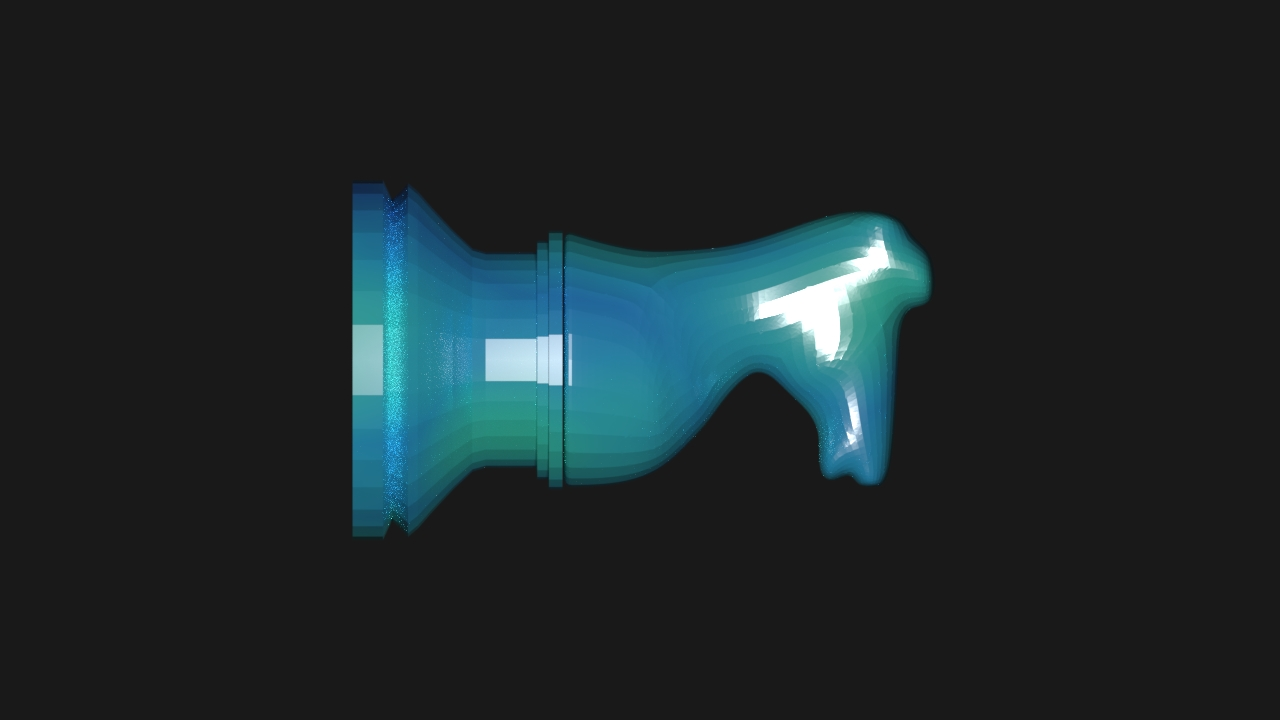
\includegraphics[width=0.33\textwidth]{interp/synth_data/knight/knight_ps}\\
  MVS & PS\\
  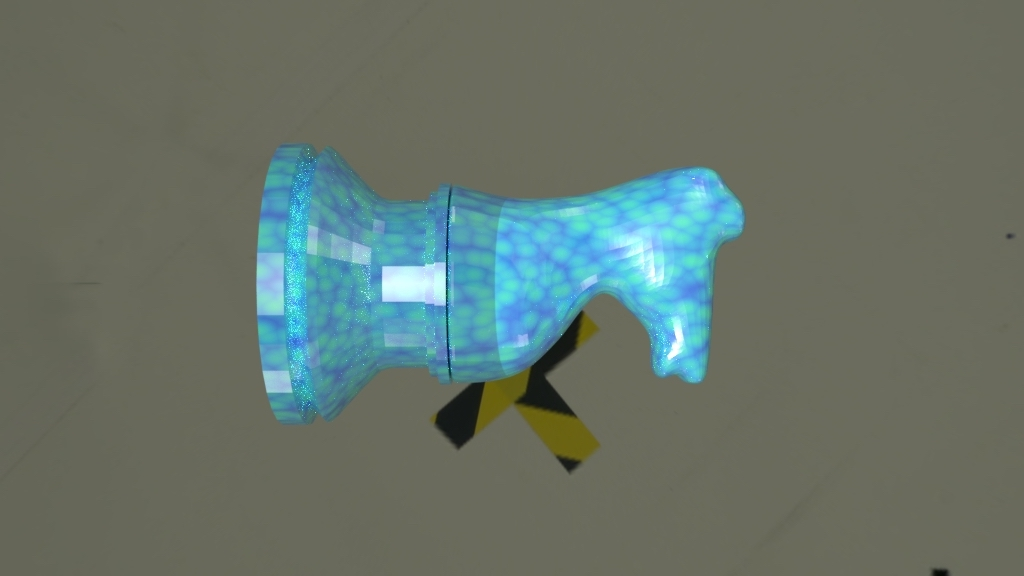
\includegraphics[width=0.33\textwidth]{interp/synth_data/knight/knight_sl}&
  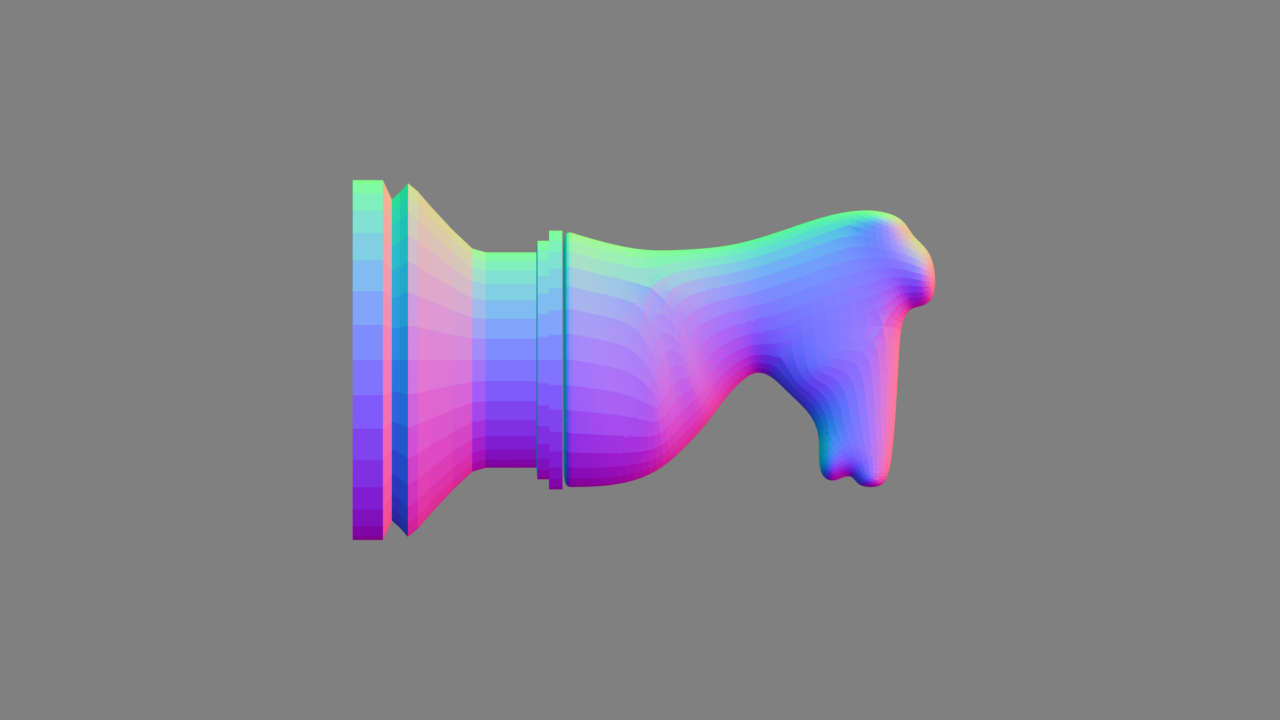
\includegraphics[width=0.33\textwidth]{interp/synth_data/knight/knight_ps_gt}\\
  SL & Normal groundtruth\\
\end{tabular}
\caption{The synthetic datasets and groundtruth for the evaluation}
\label{fig:synth_data}
\end{figure}

Now we show both the quantitative results and qualitative results of the test objects, and see if the results is consistent with the techniques selected by our abstraction.
\begin{figure}[!htbp]
\centering
\begin{tabular}{ccccc}
  Quantitative results & ~ & Qualitative results & ~\\
  \includegraphics[width=0.25\textwidth]{interp/synth_data/knight/knight_02080208}&
  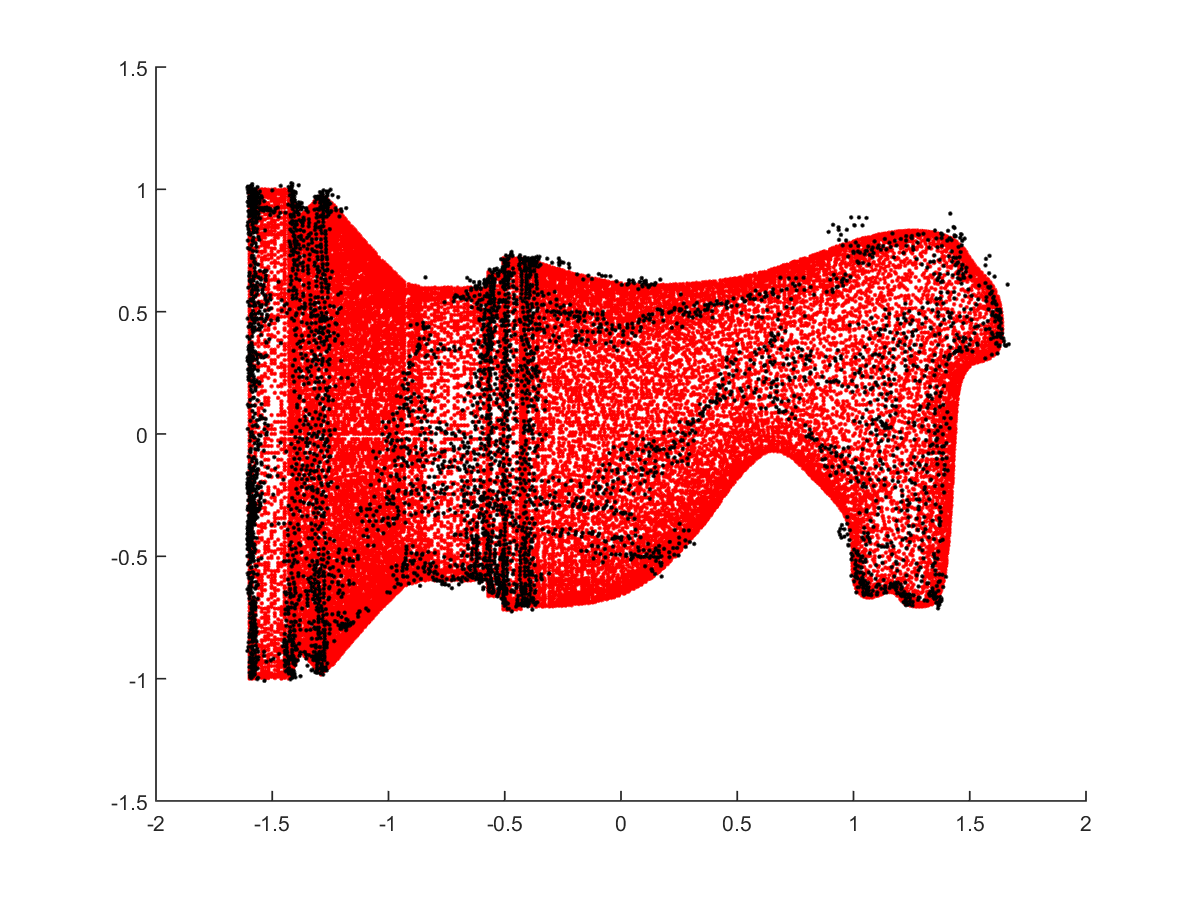
\includegraphics[width=0.25\textwidth]{interp/synth_data/knight/knight_mvs_02080208.png}&
  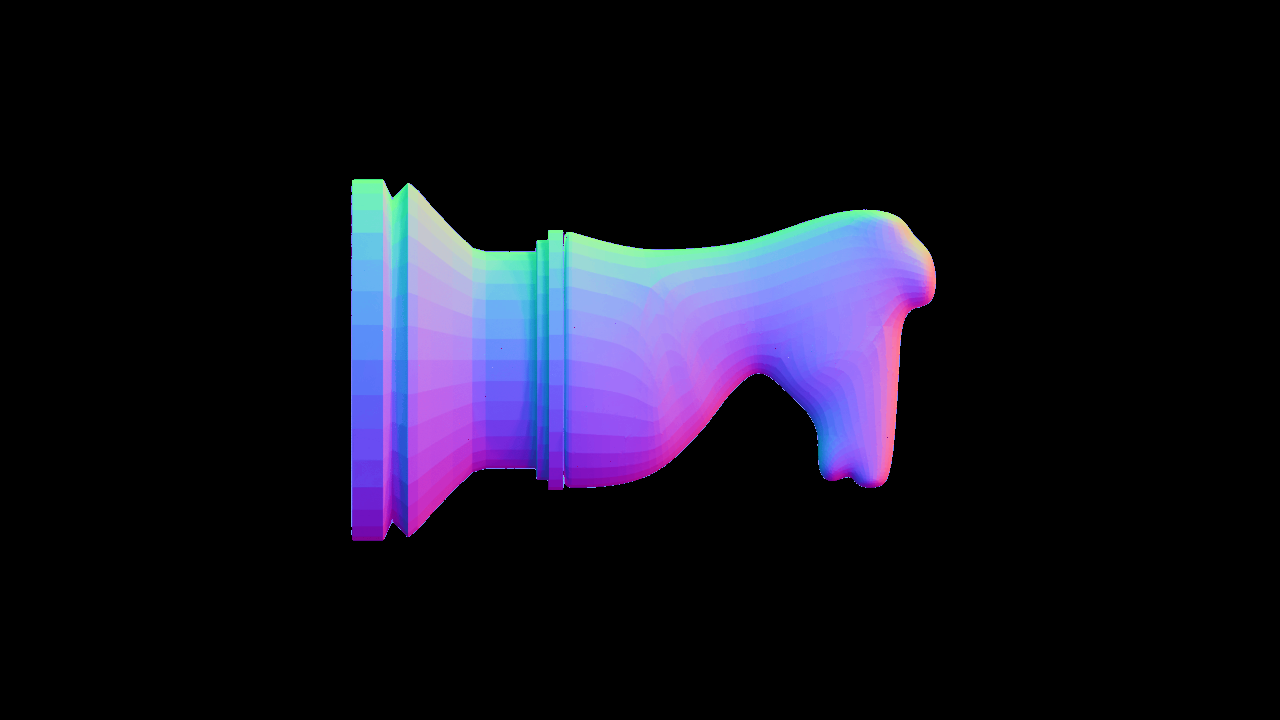
\includegraphics[width=0.25\textwidth]{interp/synth_data/knight/knight_ps_02080208.png}&
  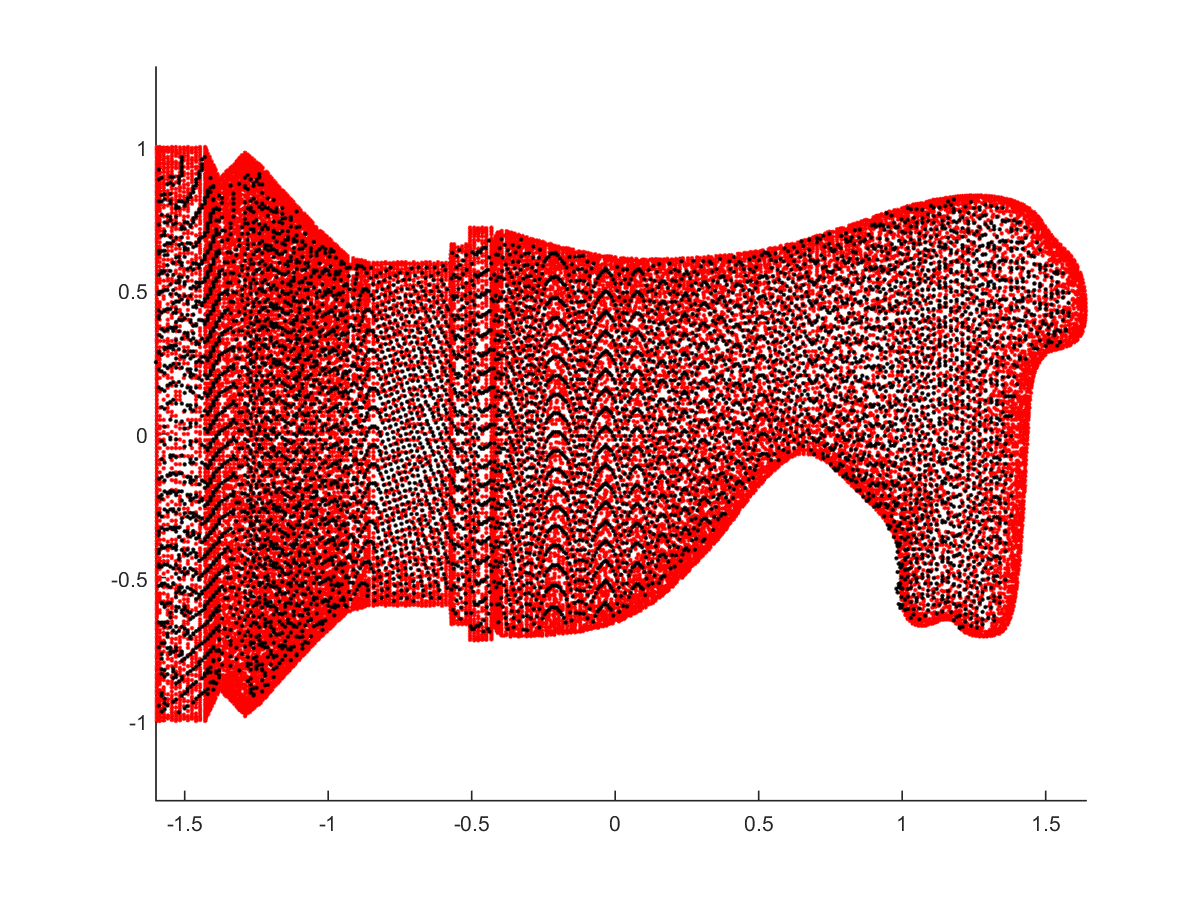
\includegraphics[width=0.25\textwidth]{interp/synth_data/knight/knight_sl_02080208.png}\\
  \multicolumn{4}{c}{(a). tex(0.2), alb(0.8), spec(0.2), rough(0.8)}\\
  \includegraphics[width=0.25\textwidth]{interp/synth_data/knight/knight_02080502}&
  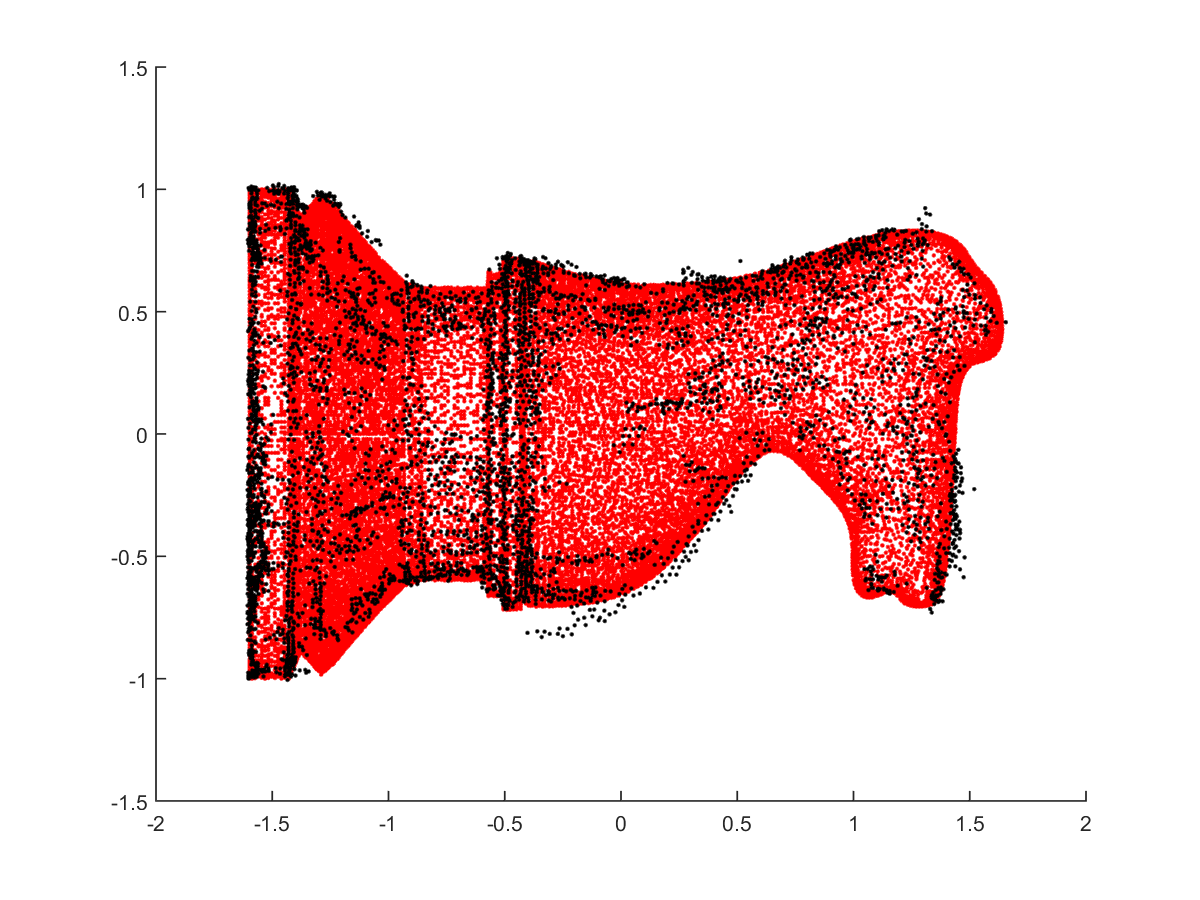
\includegraphics[width=0.25\textwidth]{interp/synth_data/knight/knight_mvs_02080502.png}&
  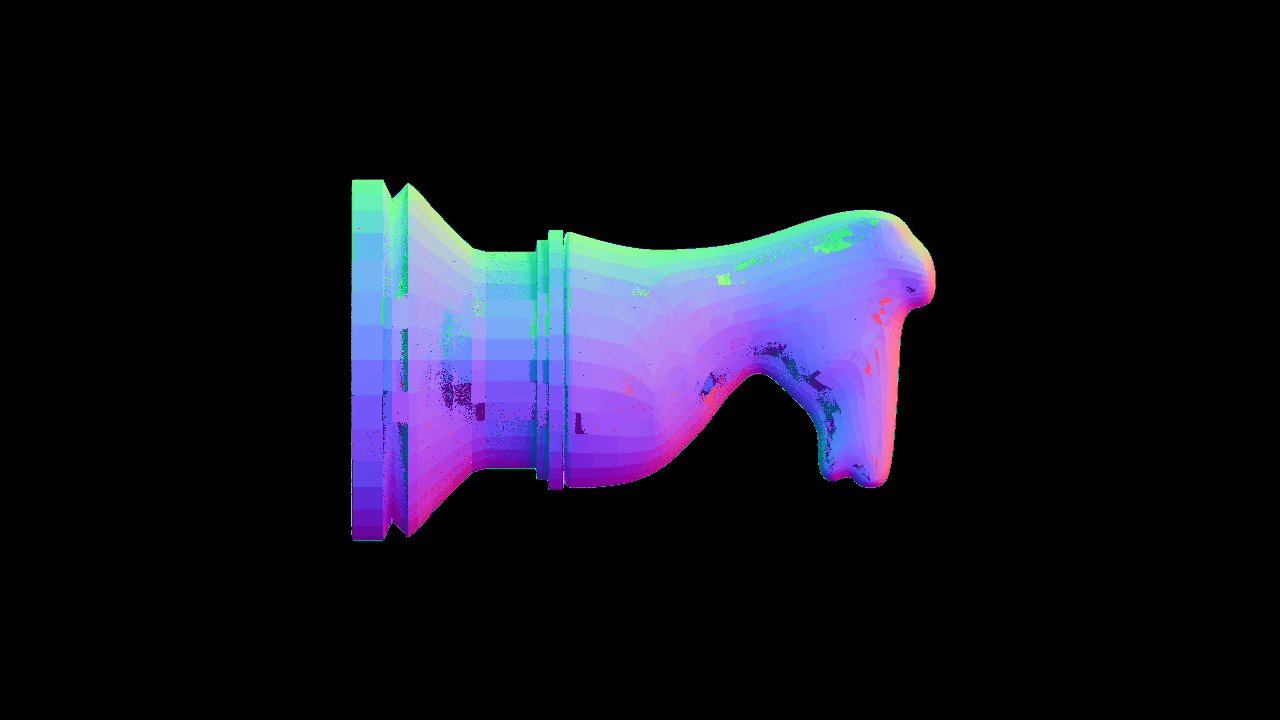
\includegraphics[width=0.25\textwidth]{interp/synth_data/knight/knight_ps_02080502.png}&
  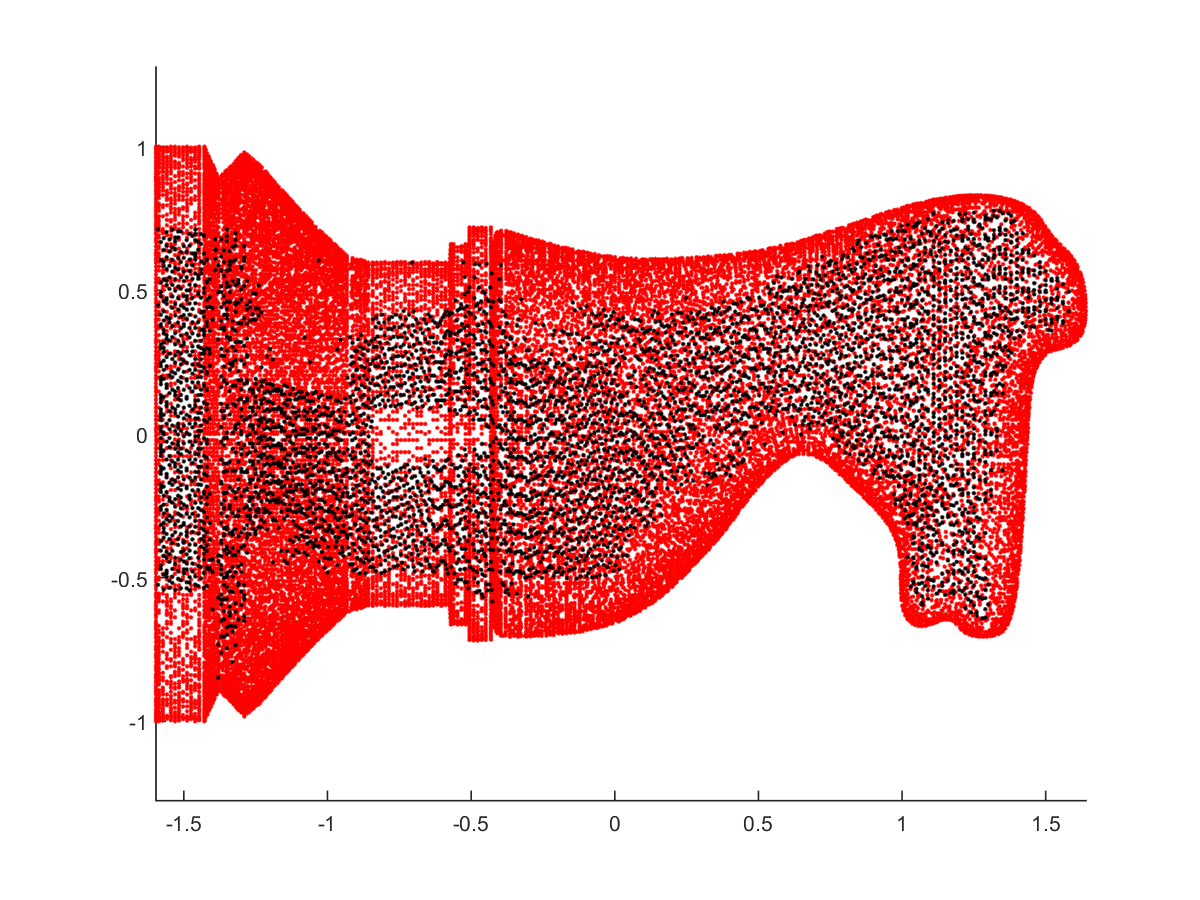
\includegraphics[width=0.25\textwidth]{interp/synth_data/knight/knight_sl_02080502.png}\\
  \multicolumn{4}{c}{(b). tex(0.2), alb(0.8), spec(0.5), rough(0.2)}\\
  \includegraphics[width=0.25\textwidth]{interp/synth_data/knight/knight_08080208}&
  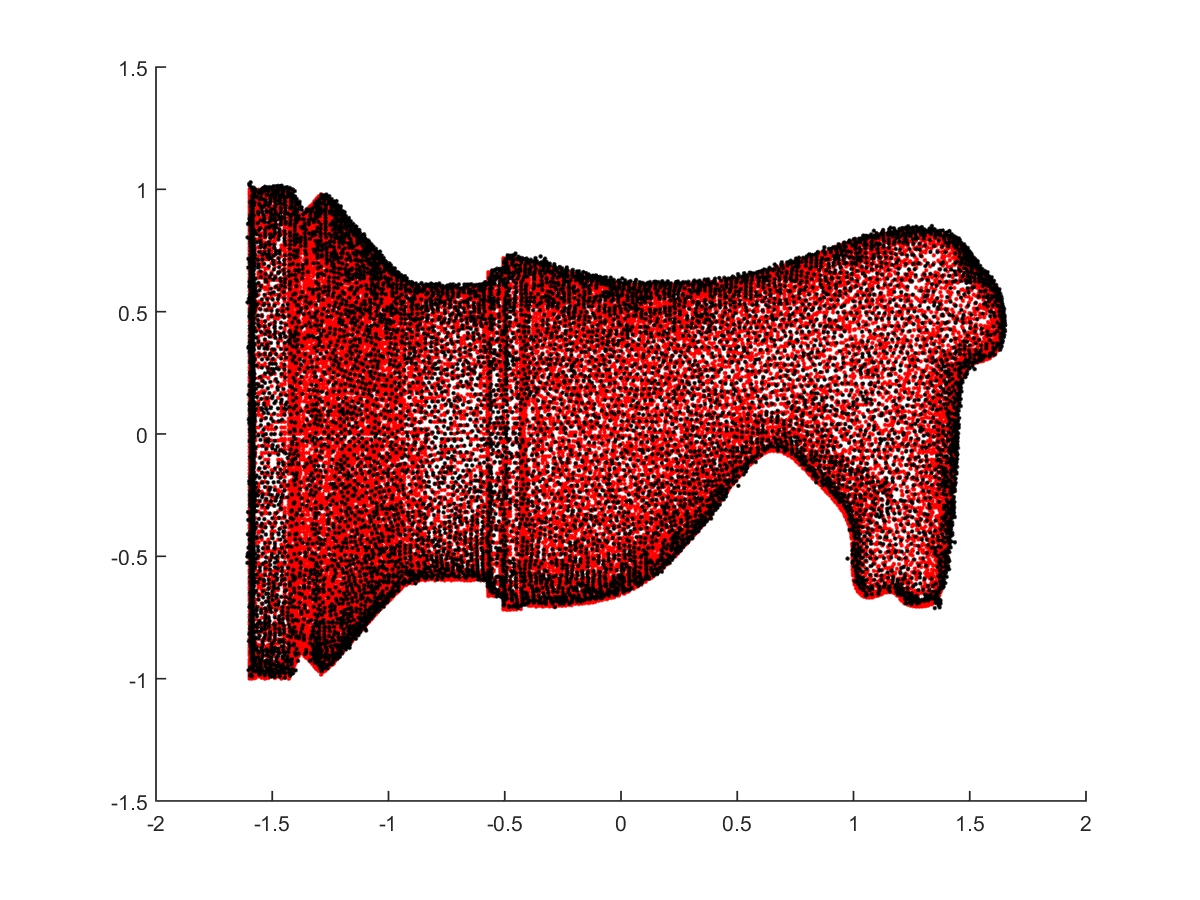
\includegraphics[width=0.25\textwidth]{interp/synth_data/knight/knight_mvs_08080208.png}&
  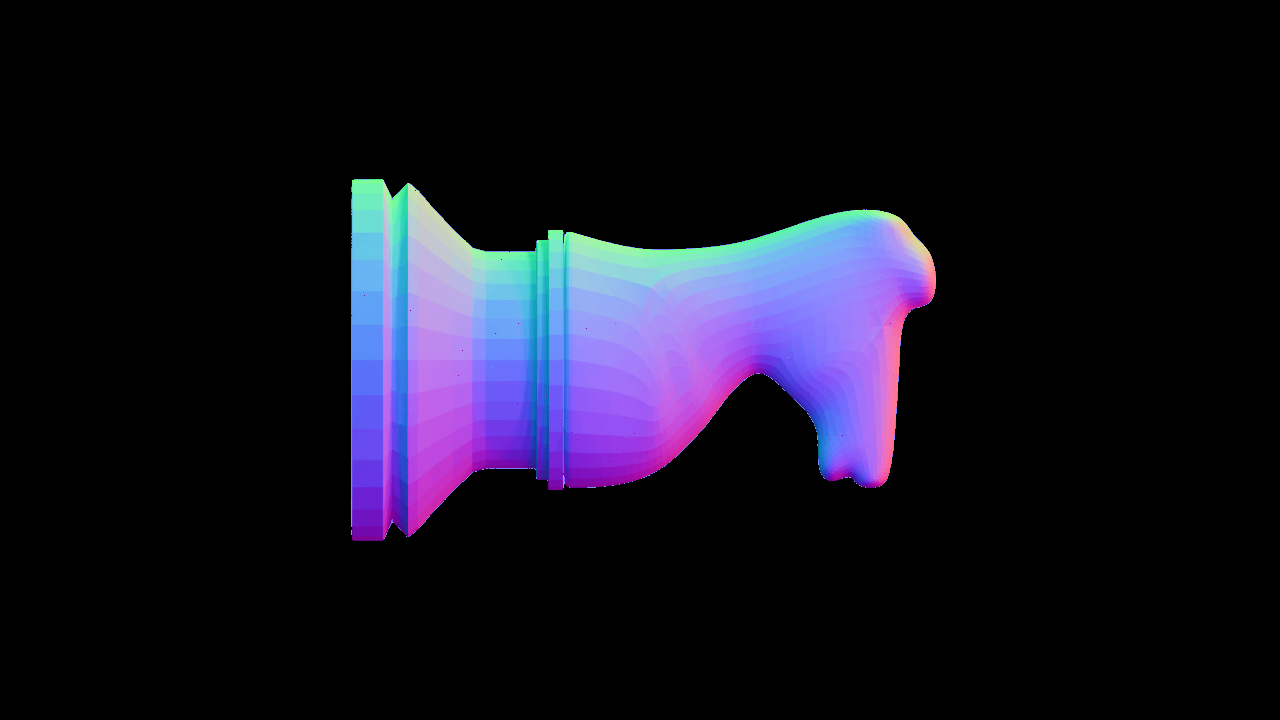
\includegraphics[width=0.25\textwidth]{interp/synth_data/knight/knight_ps_08080208.png}&
  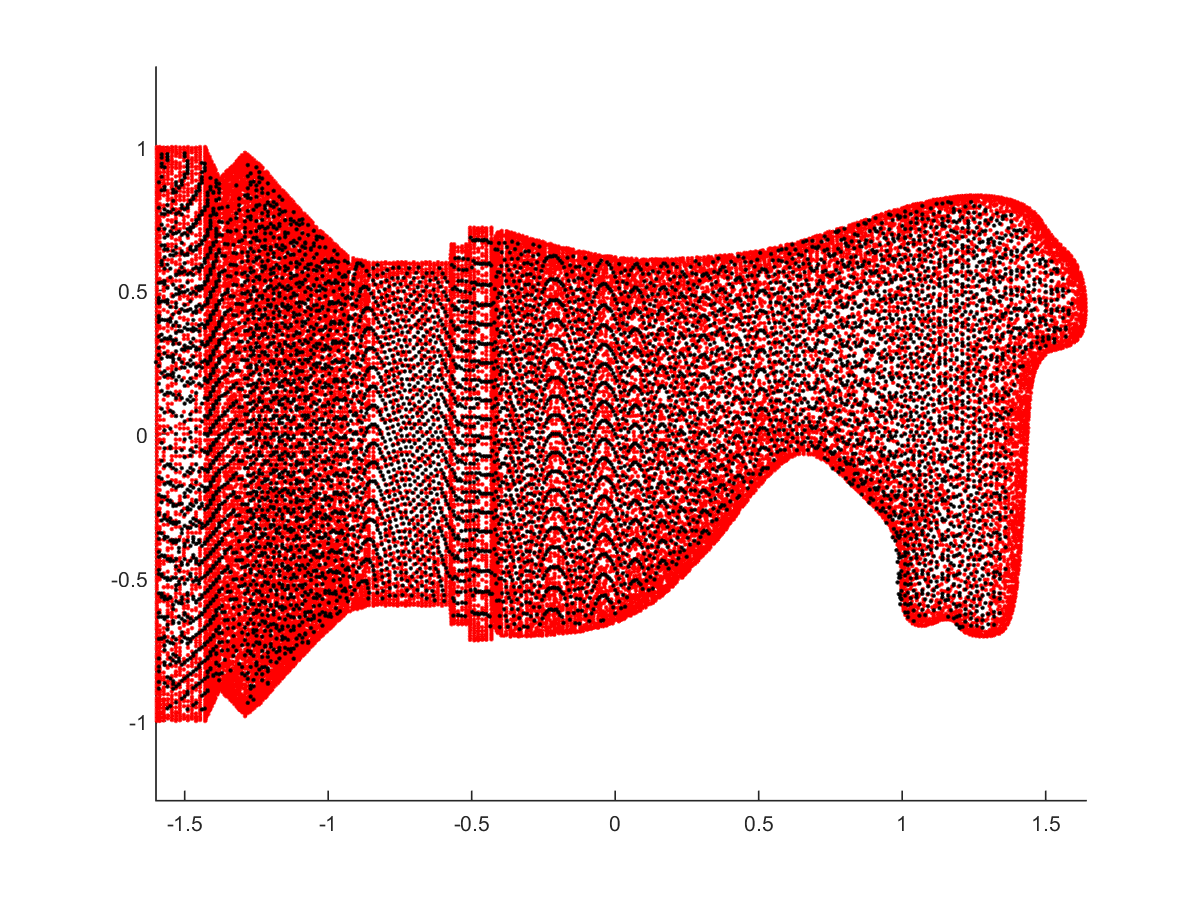
\includegraphics[width=0.25\textwidth]{interp/synth_data/knight/knight_sl_08080208.png}\\
  \multicolumn{4}{c}{(c). tex(0.8), alb(0.8), spec(0.2), rough(0.8)}\\
  \includegraphics[width=0.25\textwidth]{interp/synth_data/knight/knight_08080502}&
  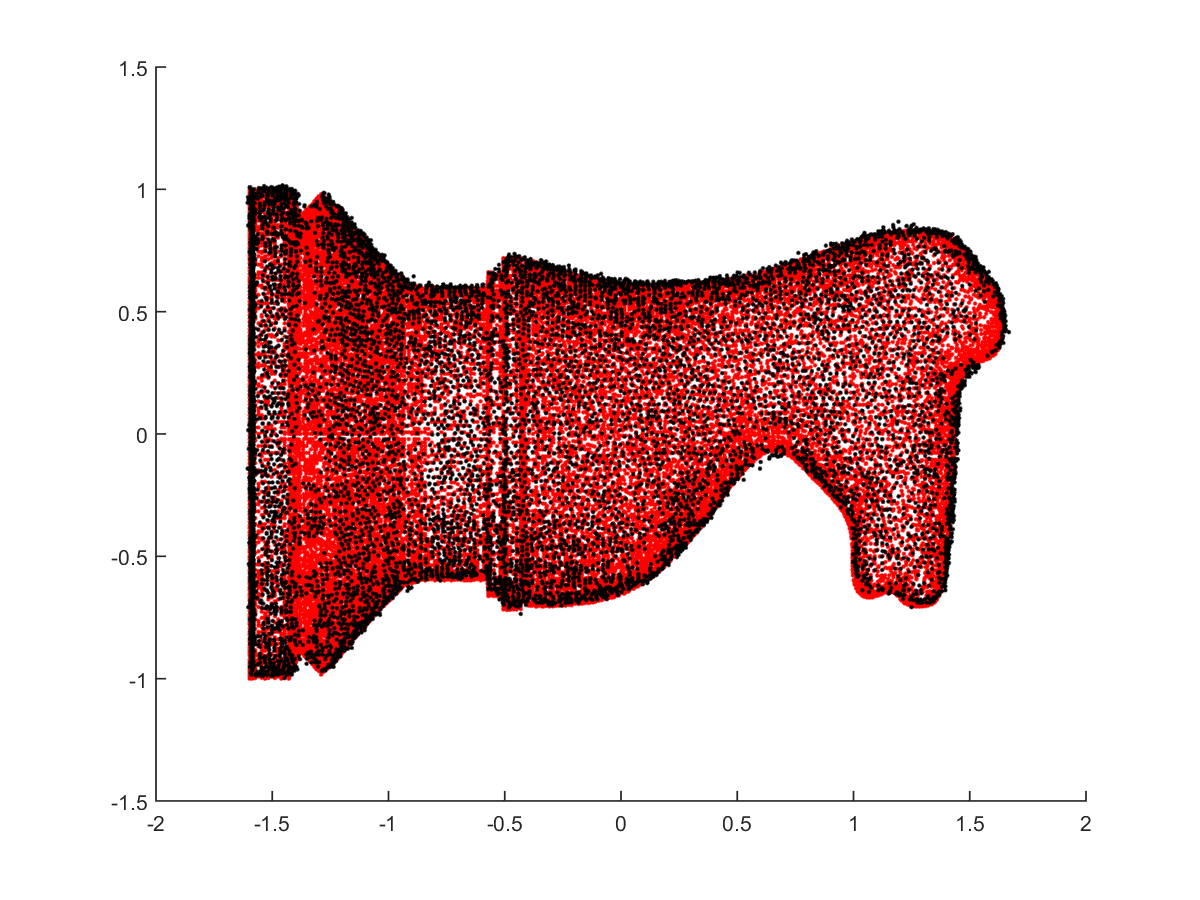
\includegraphics[width=0.25\textwidth]{interp/synth_data/knight/knight_mvs_08080502.png}&
  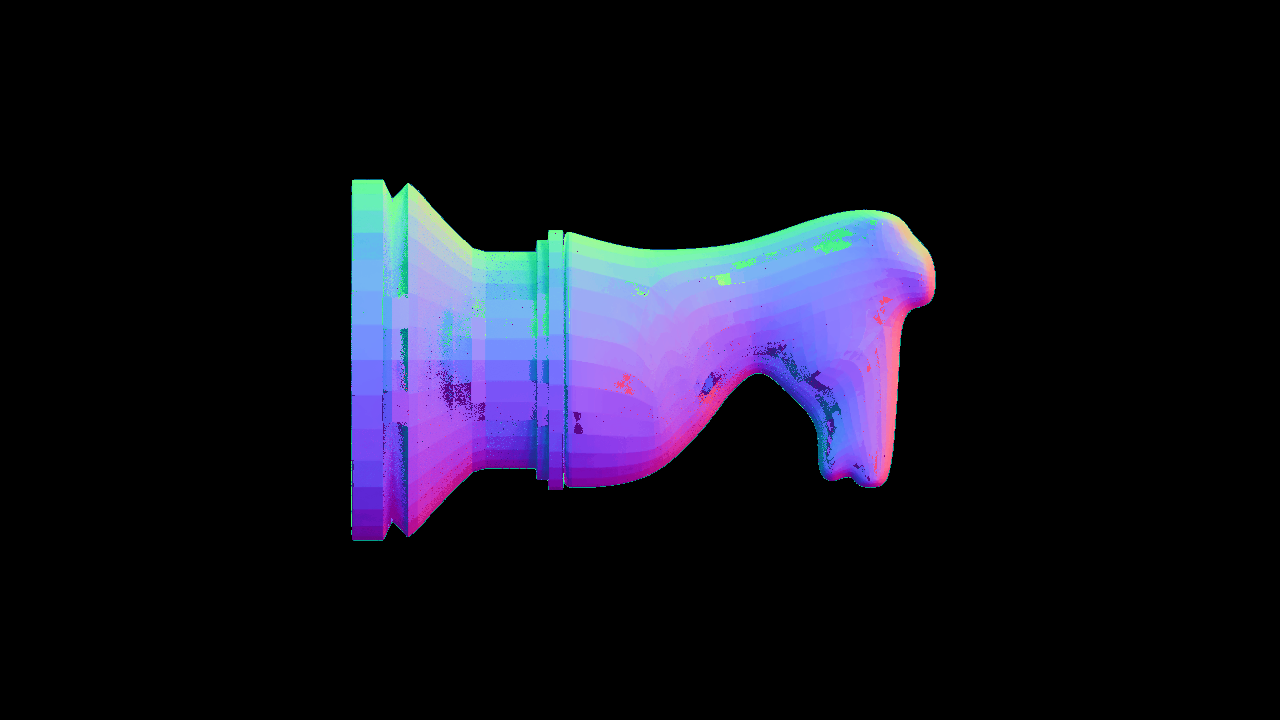
\includegraphics[width=0.25\textwidth]{interp/synth_data/knight/knight_ps_08080502.png}&
  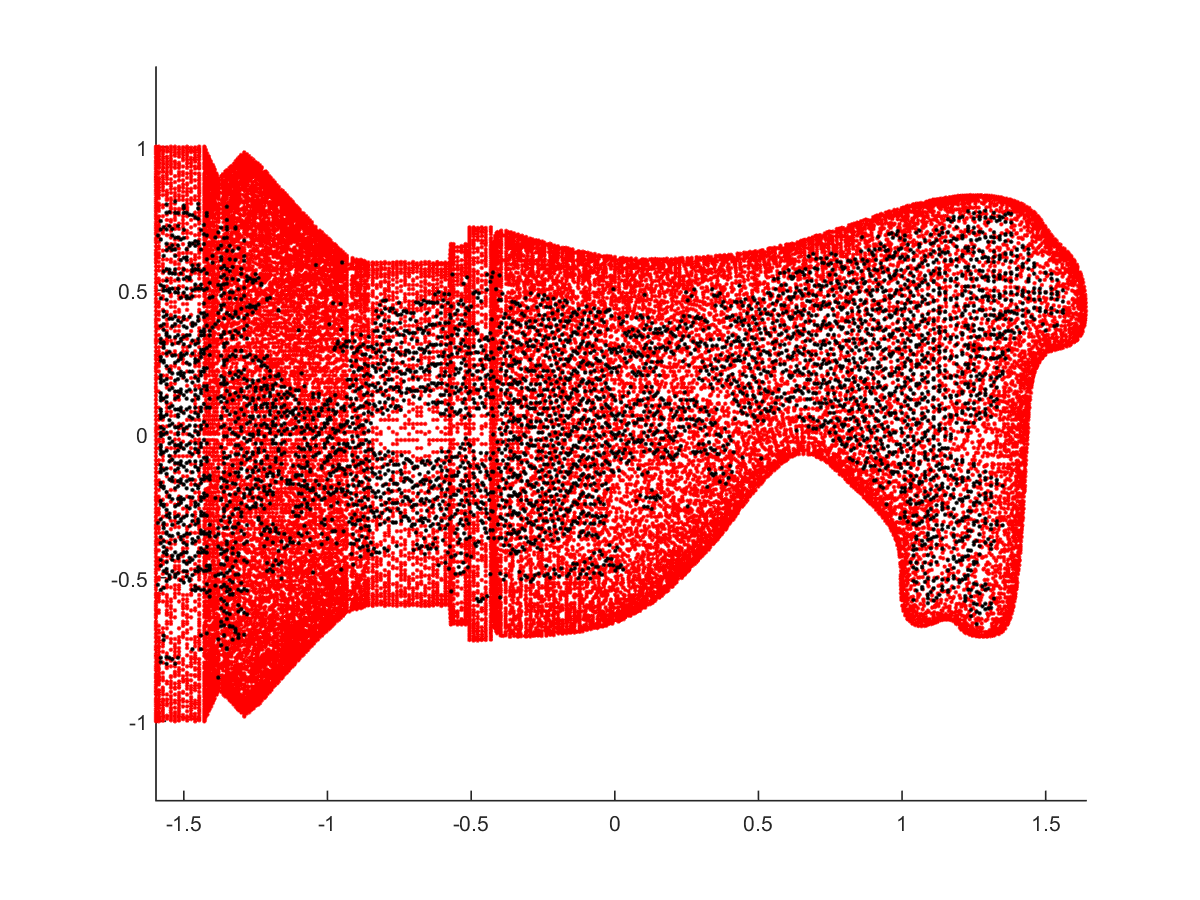
\includegraphics[width=0.25\textwidth]{interp/synth_data/knight/knight_sl_08080502.png}\\
  \multicolumn{4}{c}{(d). tex(0.8), alb(0.8), spec(0.5), rough(0.2)}\\
  ~ & MVS & PS & SL\\
\end{tabular}
\caption{The quantitative and qualitative performance of each technique on the synthetic dataset. The red dots are from the ground truth while the black ones the reconstruction.}
\label{fig:synth_data_results}
\end{figure}

\textbf{Case 1\&2} Both example-based PS and Gray coded SL perform relatively well, as suggested by the mapping. The completeness of the PMVS is low due to the lack of texture. The results are consistent to those returned by the mapping which is shown in Table~\ref{tab:prop_list} (a) and (b).

\textbf{Case 3\&4} All three algorithms perform relatively well, which is also consistent to the results returned by the mapping, as shown in Table~\ref{tab:prop_list_synth_data} (c) - (d).

\section{Real-world Datasets}
We used a similar setup to the synthetic settings and captured a real world dataset for nine objects. The property of these objects are listed in Table~\ref{tab:prop_list_real_data}.

\begin{table}[!htbp]
  \centering
  \begin{tabular}{*{9}{c}}
  \multicolumn{3}{l}{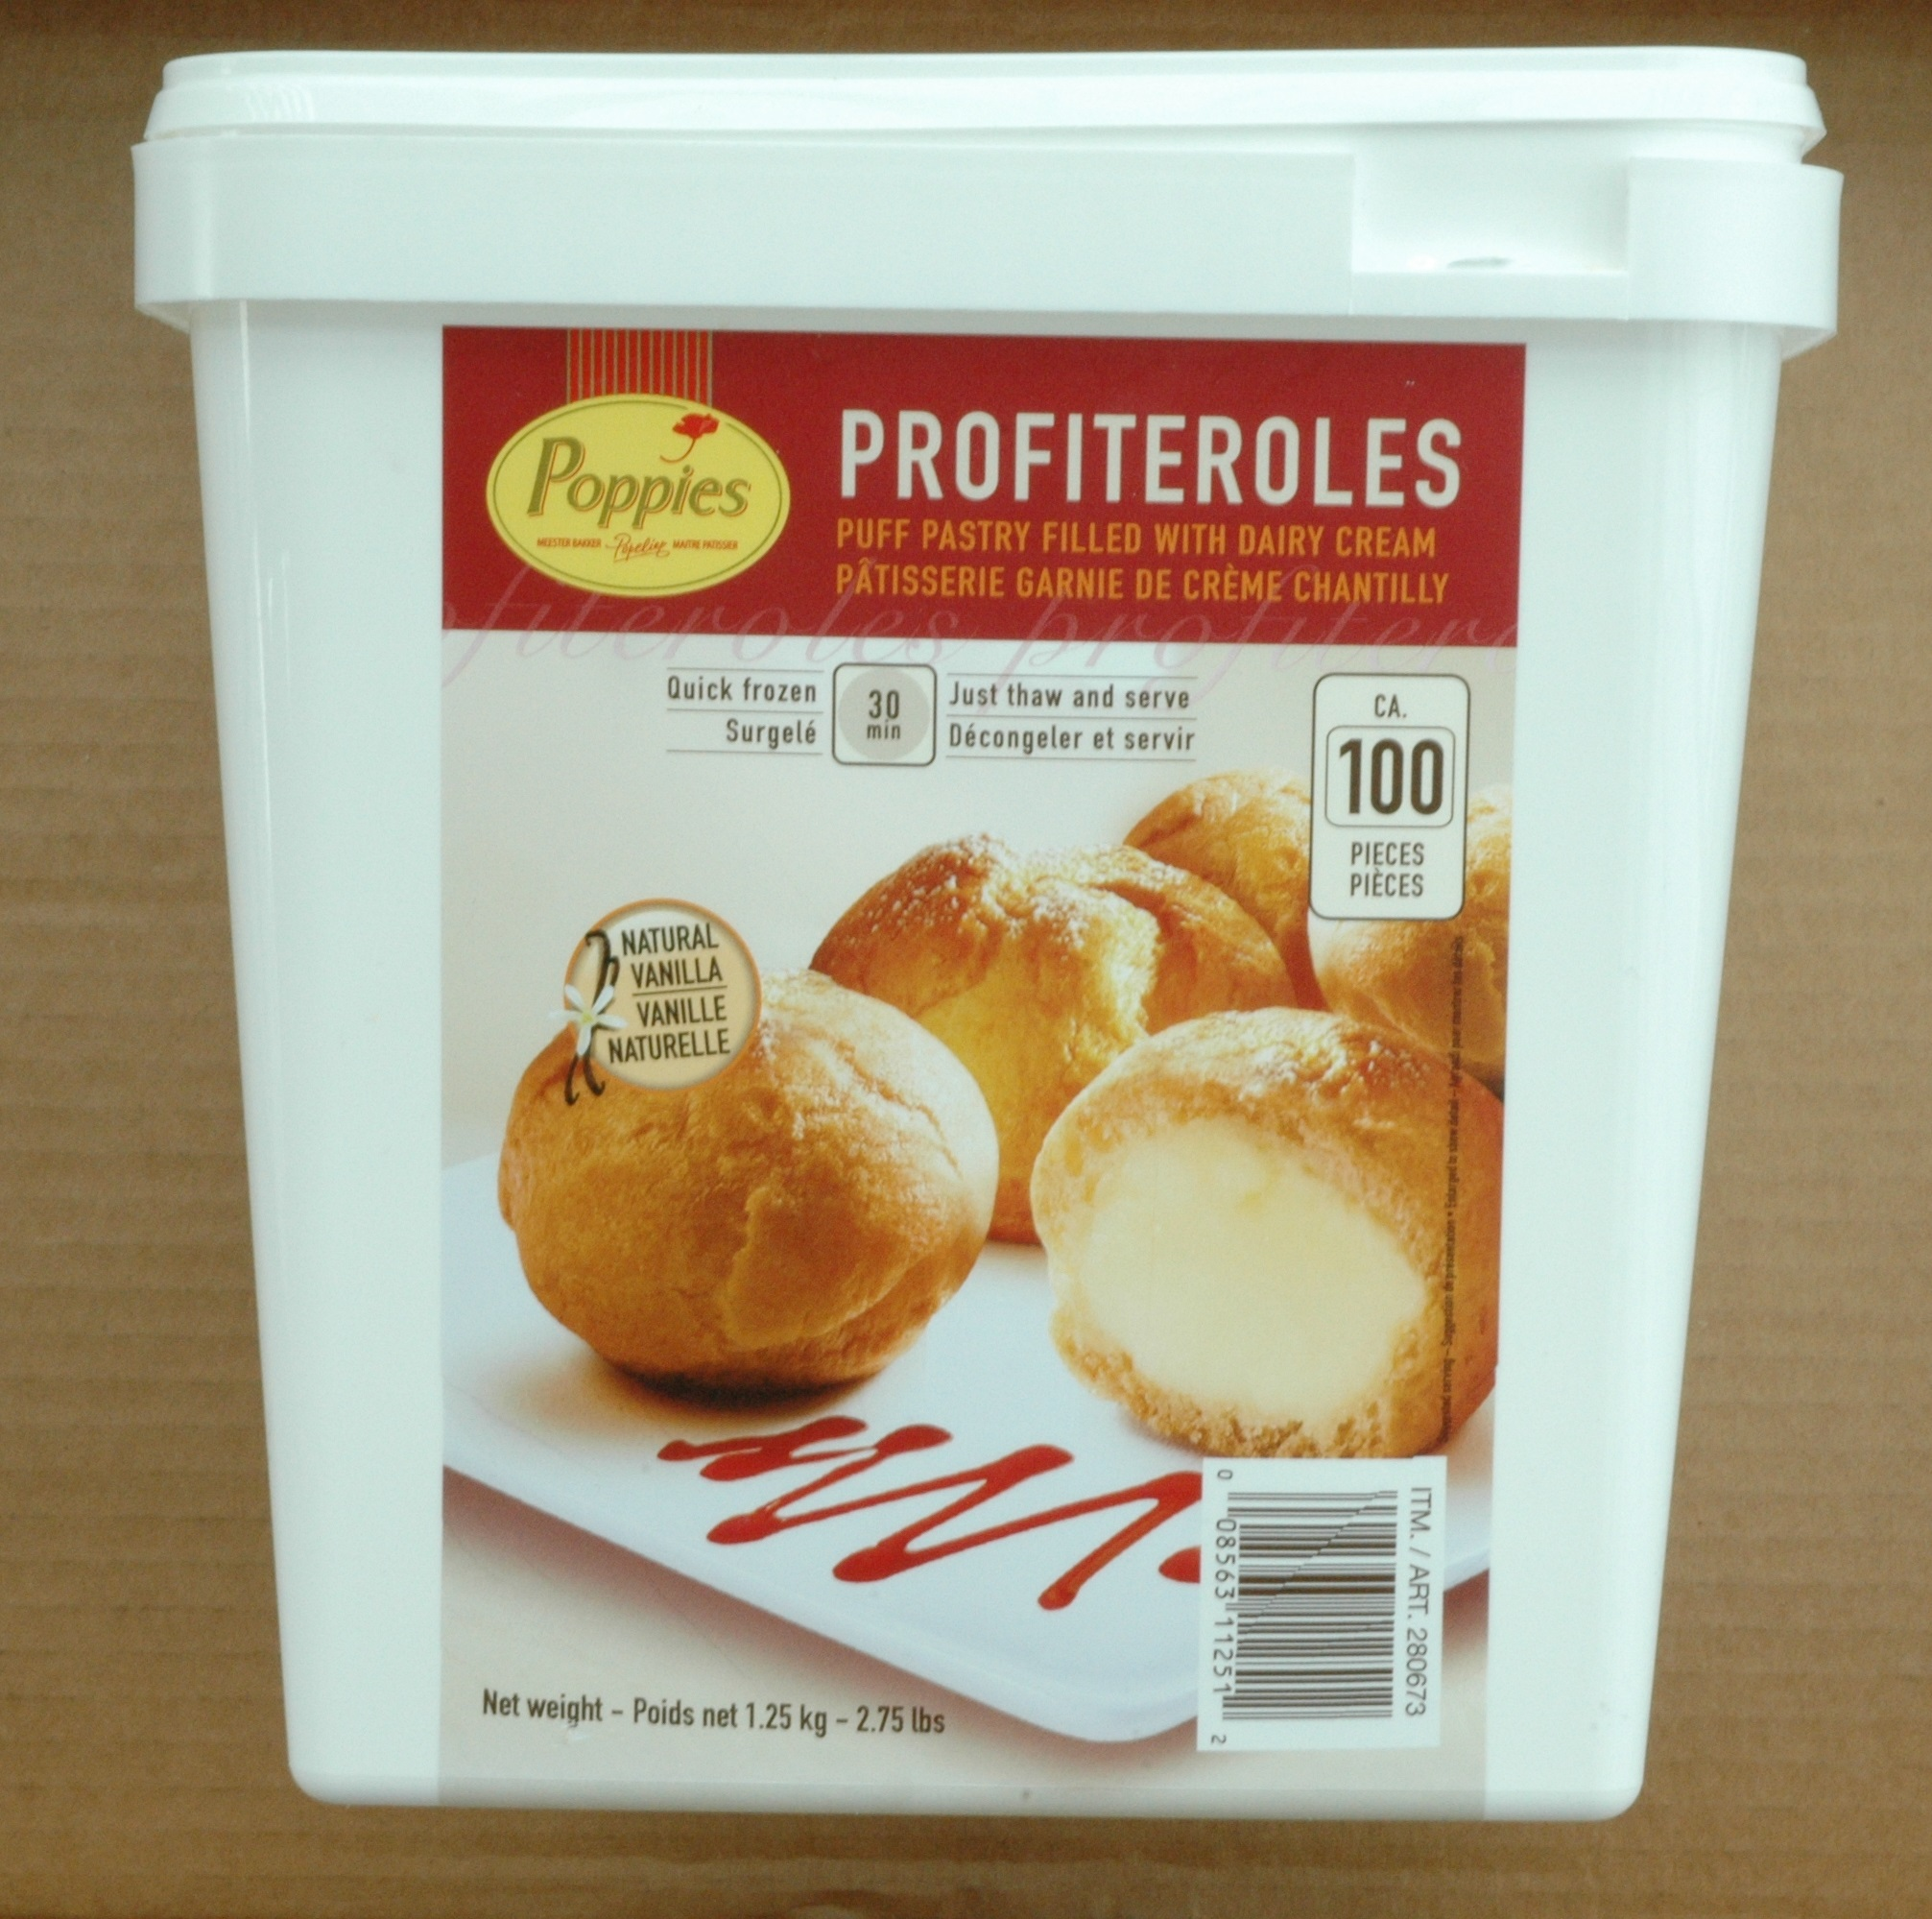
\includegraphics[width=0.33\textwidth]{interp/real_world_obj/box/box}} &
  \multicolumn{3}{l}{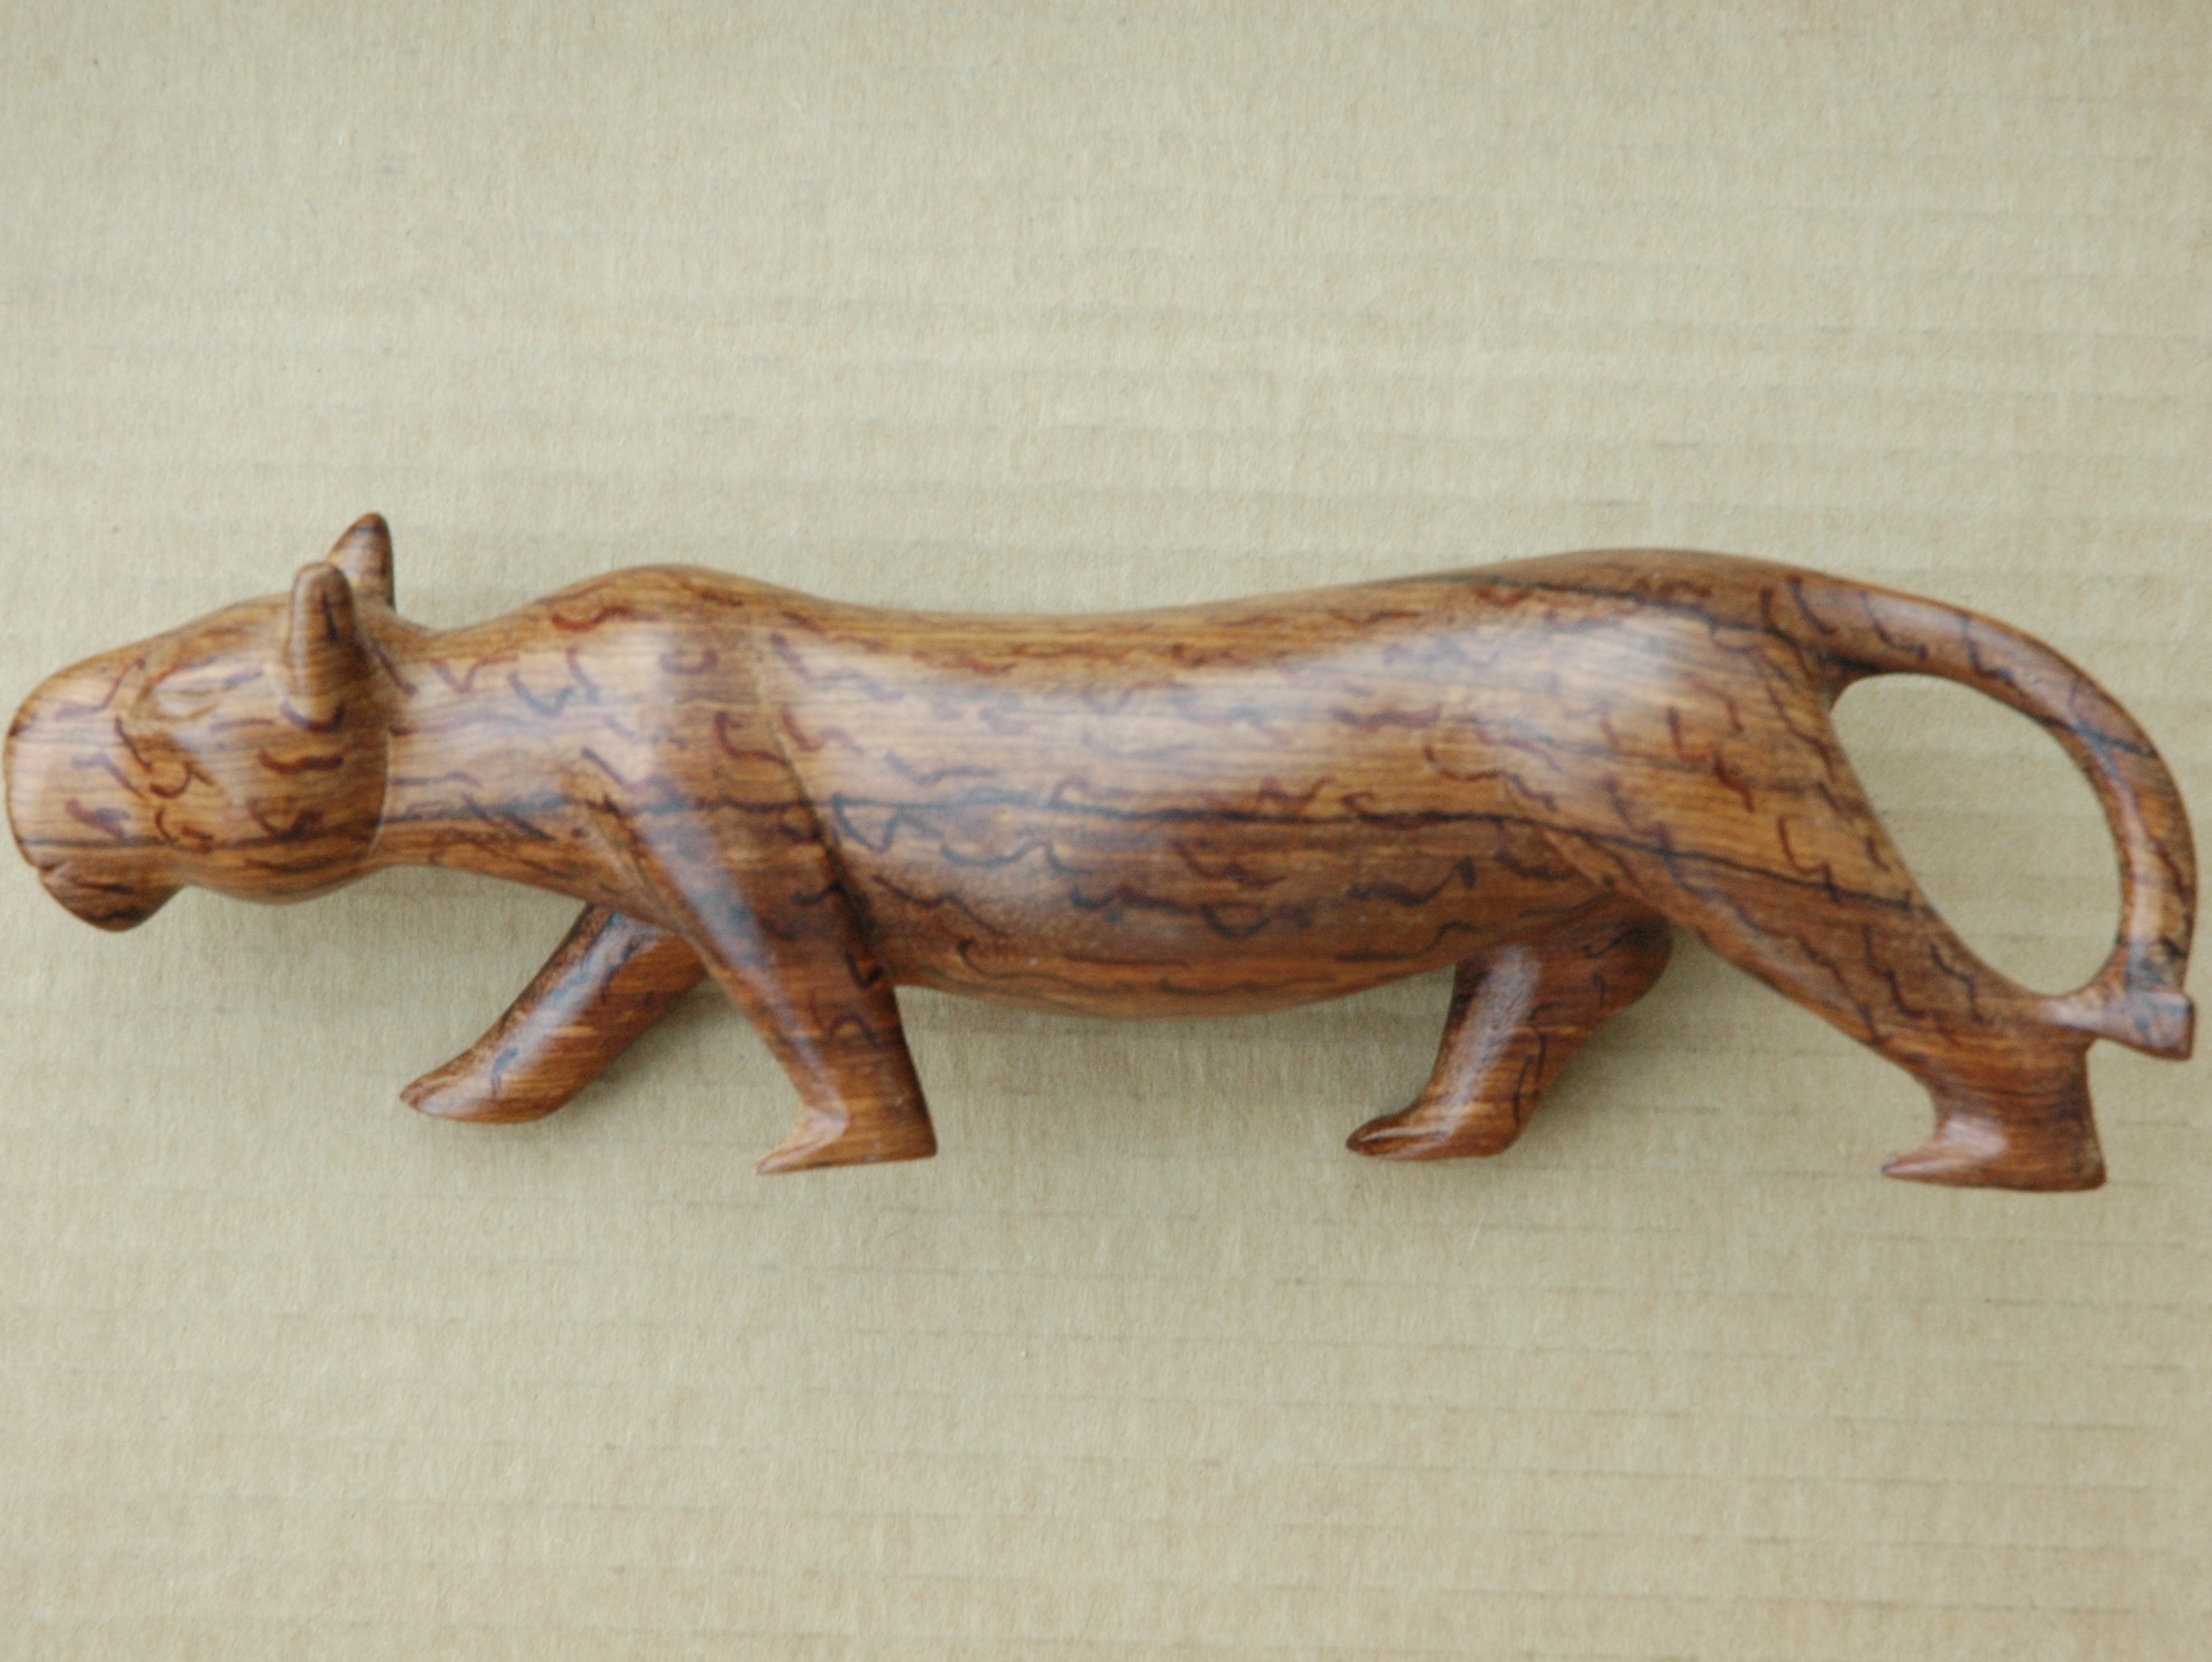
\includegraphics[width=0.33\textwidth]{interp/real_world_obj/cat0/cat0}} &
  \multicolumn{3}{l}{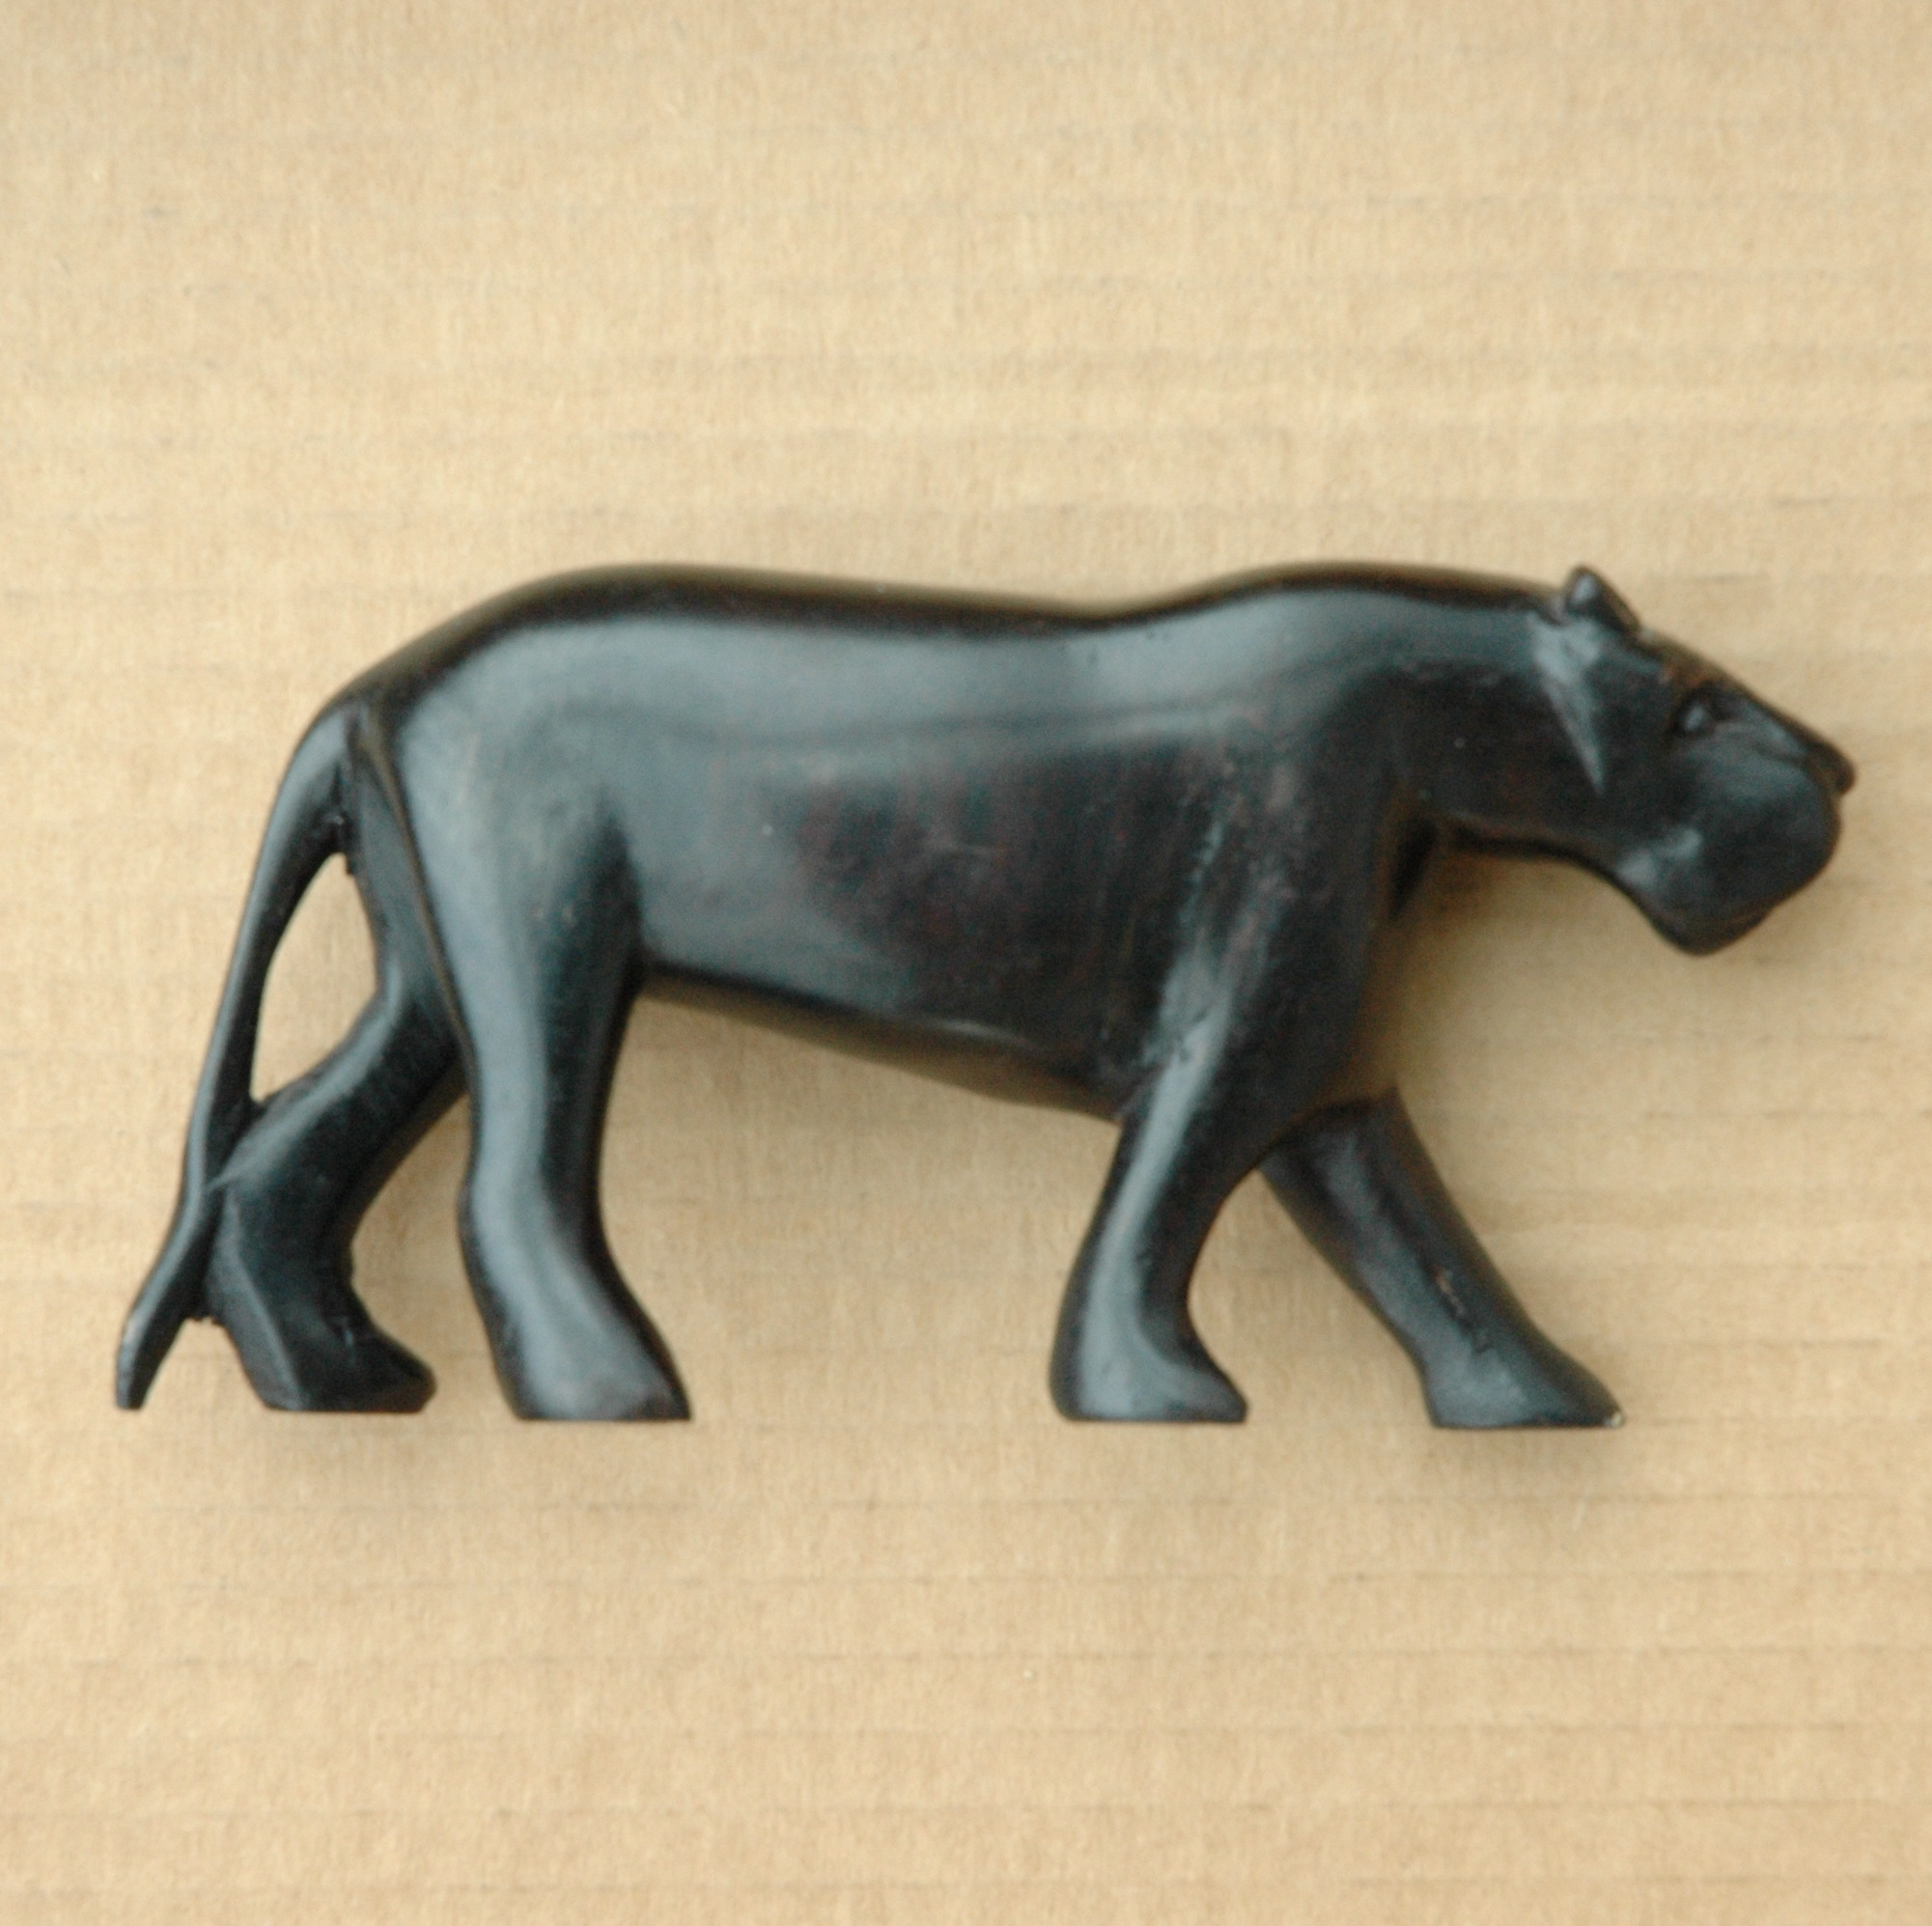
\includegraphics[width=0.33\textwidth]{interp/real_world_obj/cat1/cat1}}\\
  \includegraphics[width=0.1\textwidth]{interp/real_world_obj/box/base_00} &
  \includegraphics[width=0.1\textwidth]{interp/real_world_obj/box/base_01} & 
  \includegraphics[width=0.1\textwidth]{interp/real_world_obj/box/base_02} &
  \includegraphics[width=0.1\textwidth]{interp/real_world_obj/cat0/base_00} & 
  \includegraphics[width=0.1\textwidth]{interp/real_world_obj/cat0/base_01}& &
  \includegraphics[width=0.1\textwidth]{interp/real_world_obj/cat1/base_00} &\\
  \multicolumn{3}{c}{(a). box} & \multicolumn{3}{c}{(b). cat0} & \multicolumn{3}{c}{(c). cat1} \\
  \multicolumn{3}{l}{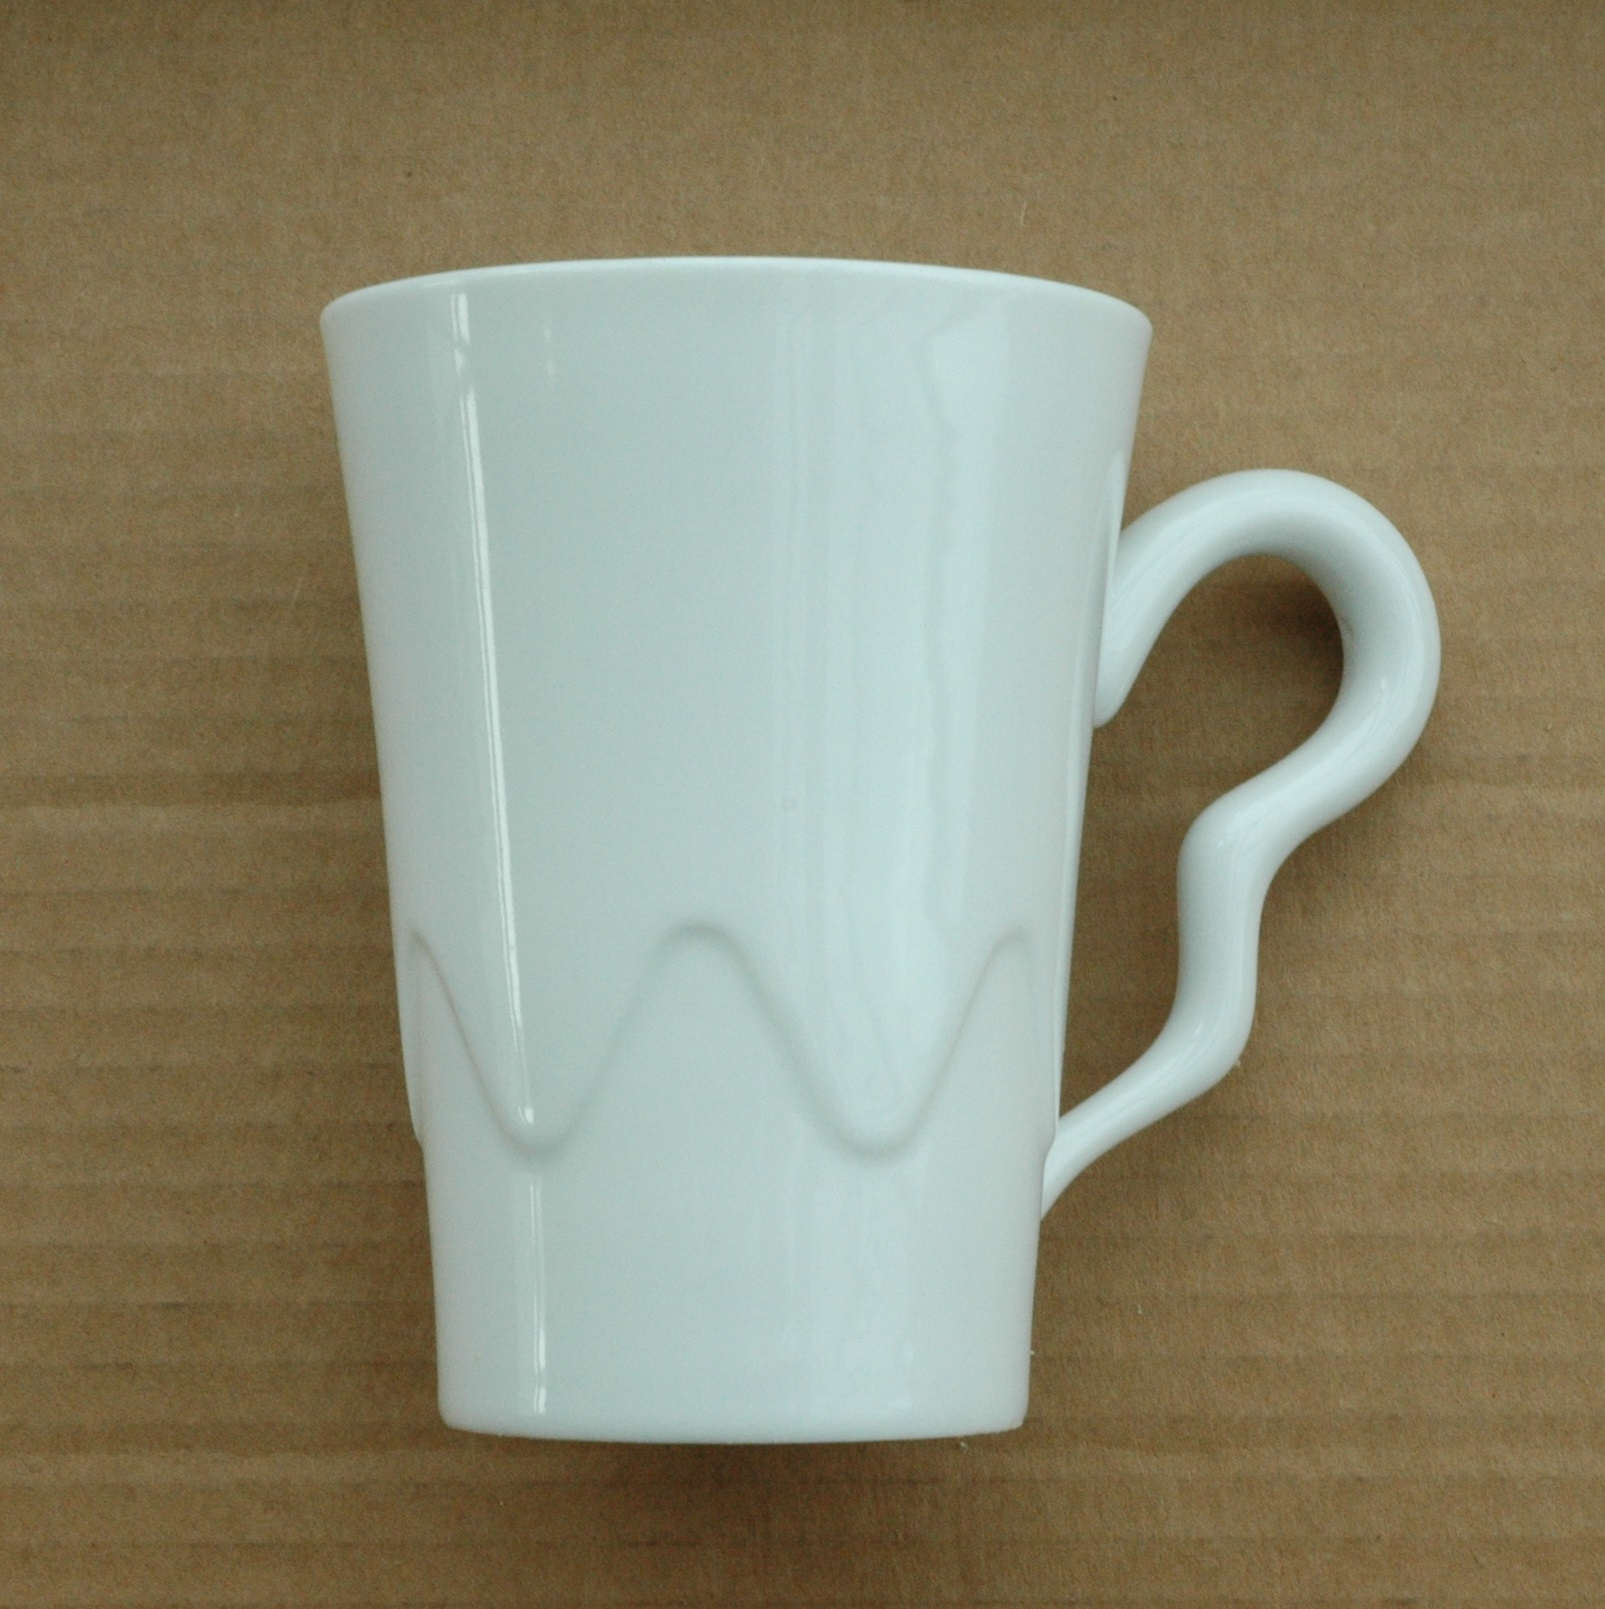
\includegraphics[width=0.33\textwidth]{interp/real_world_obj/cup/cup}} &
  \multicolumn{3}{l}{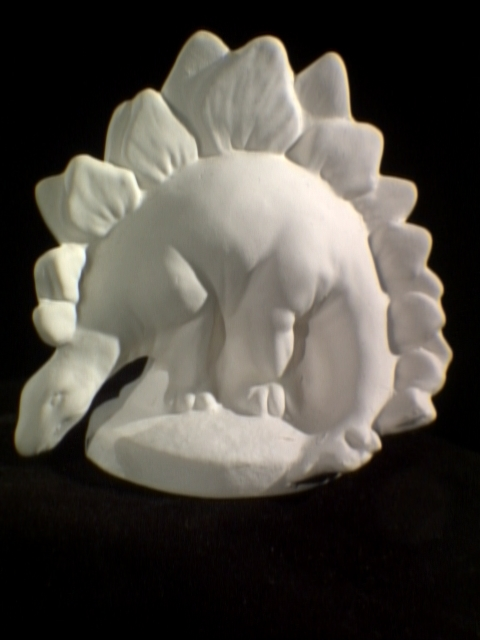
\includegraphics[width=0.33\textwidth]{interp/real_world_obj/dino/dino}} &
  \multicolumn{3}{l}{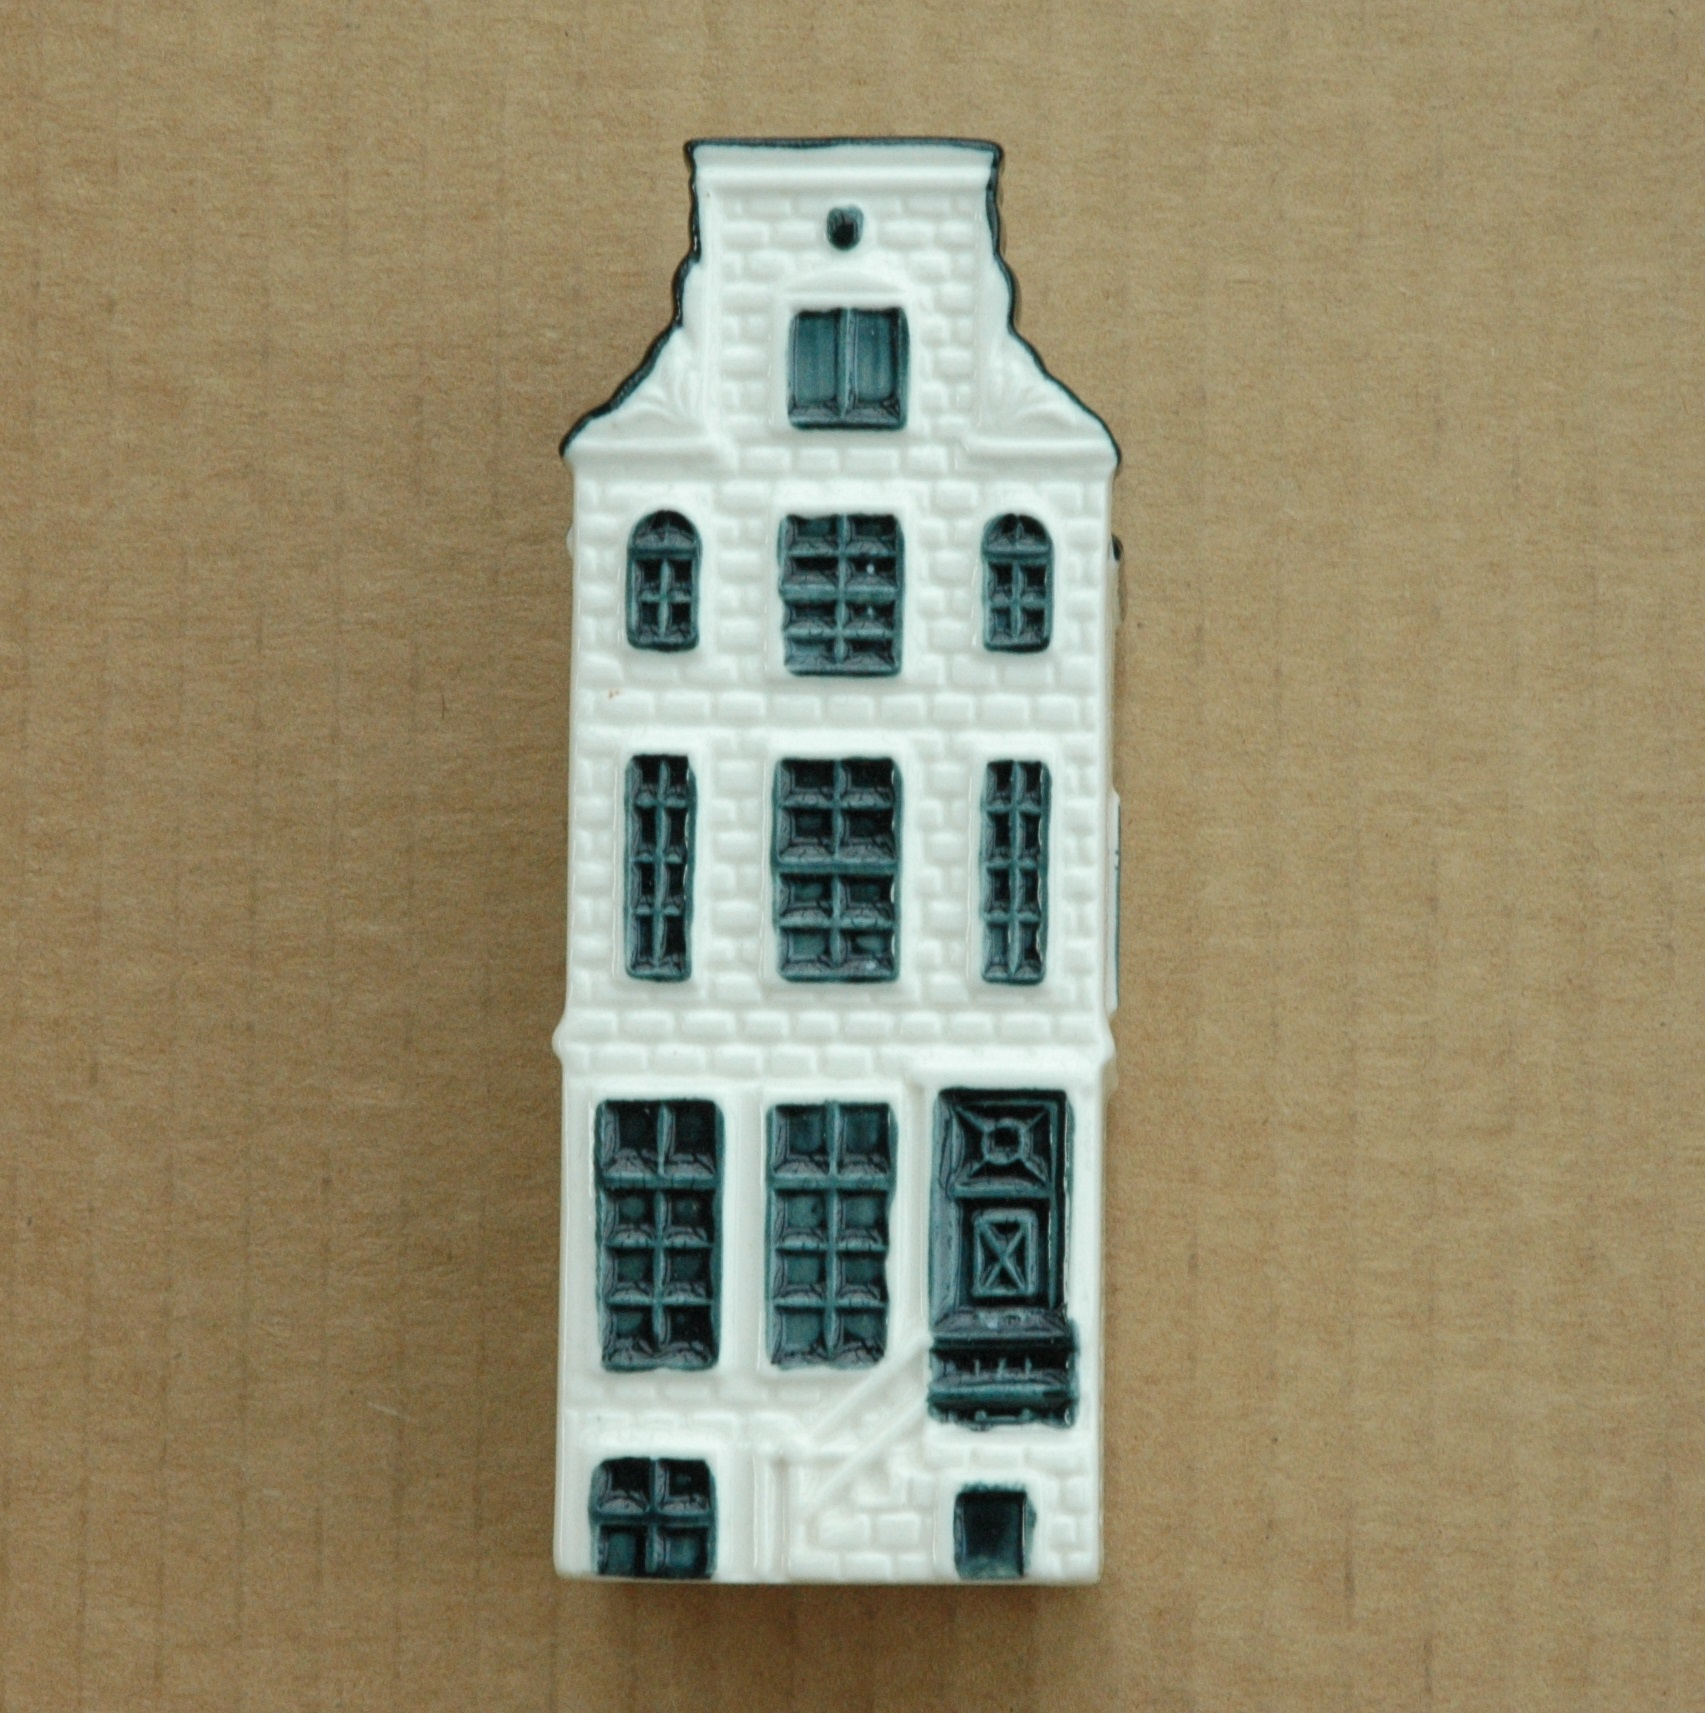
\includegraphics[width=0.33\textwidth]{interp/real_world_obj/house/house}}\\
  \includegraphics[width=0.1\textwidth]{interp/real_world_obj/cup/base_00} & & &
  \includegraphics[width=0.1\textwidth]{interp/real_world_obj/dino/base_00} & 
  \includegraphics[width=0.1\textwidth]{interp/real_world_obj/dino/base_01} & 
  \includegraphics[width=0.1\textwidth]{interp/real_world_obj/dino/base_02} &
  \includegraphics[width=0.1\textwidth]{interp/real_world_obj/house/base_00} &
  \includegraphics[width=0.1\textwidth]{interp/real_world_obj/house/base_01} & \\
  \multicolumn{3}{c}{(d). cup} & \multicolumn{3}{c}{(e). dino} & \multicolumn{3}{c}{(f). house} \\
  \multicolumn{3}{l}{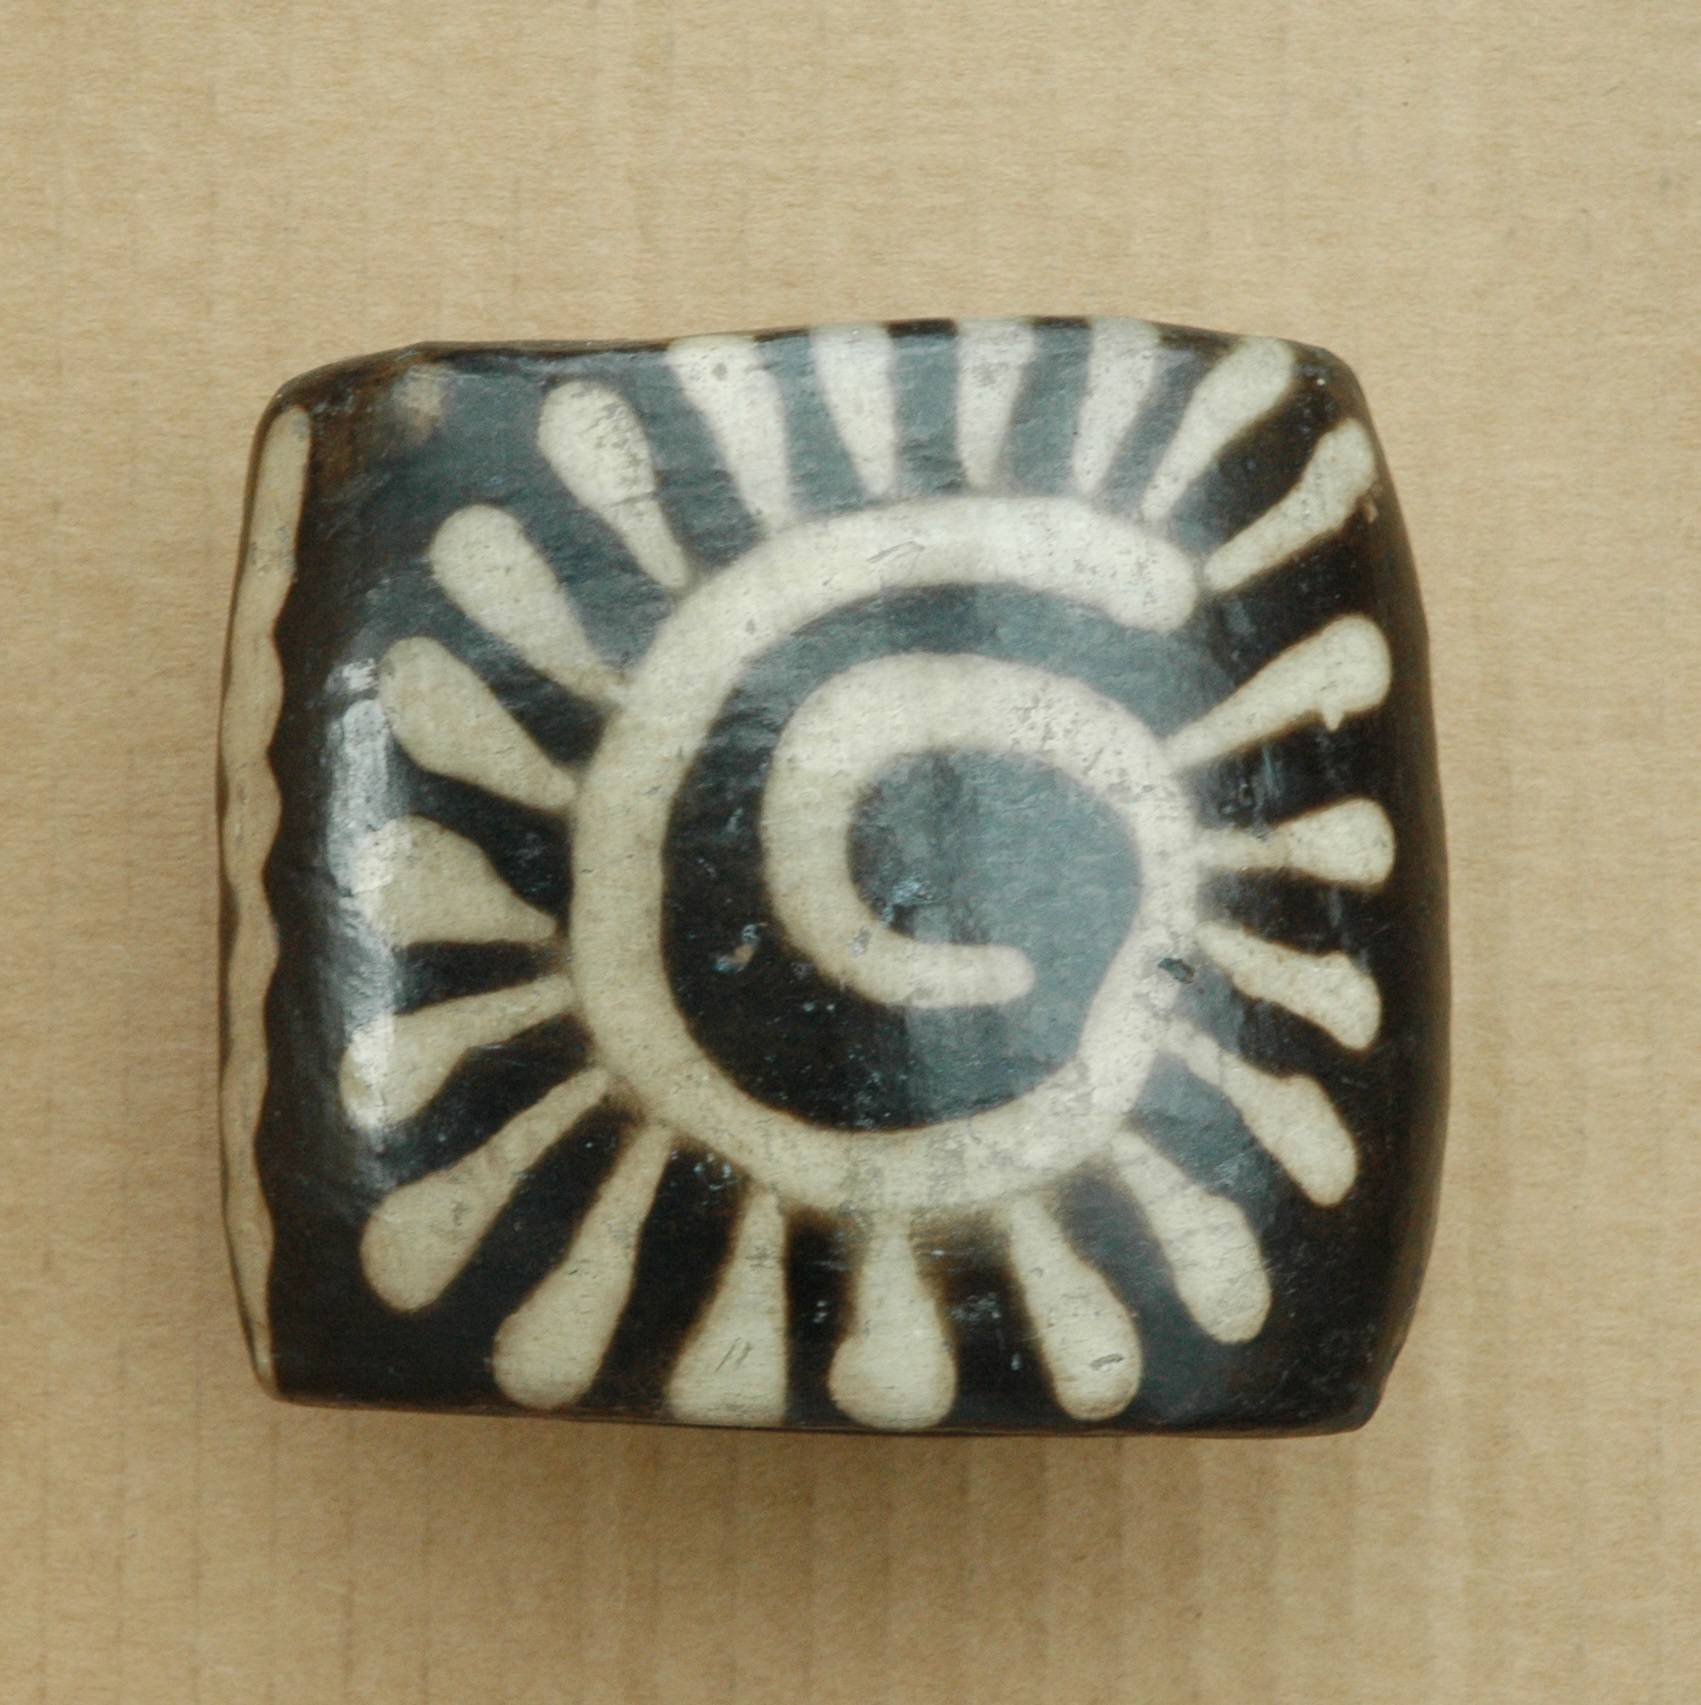
\includegraphics[width=0.33\textwidth]{interp/real_world_obj/pot/pot}} &
  \multicolumn{3}{l}{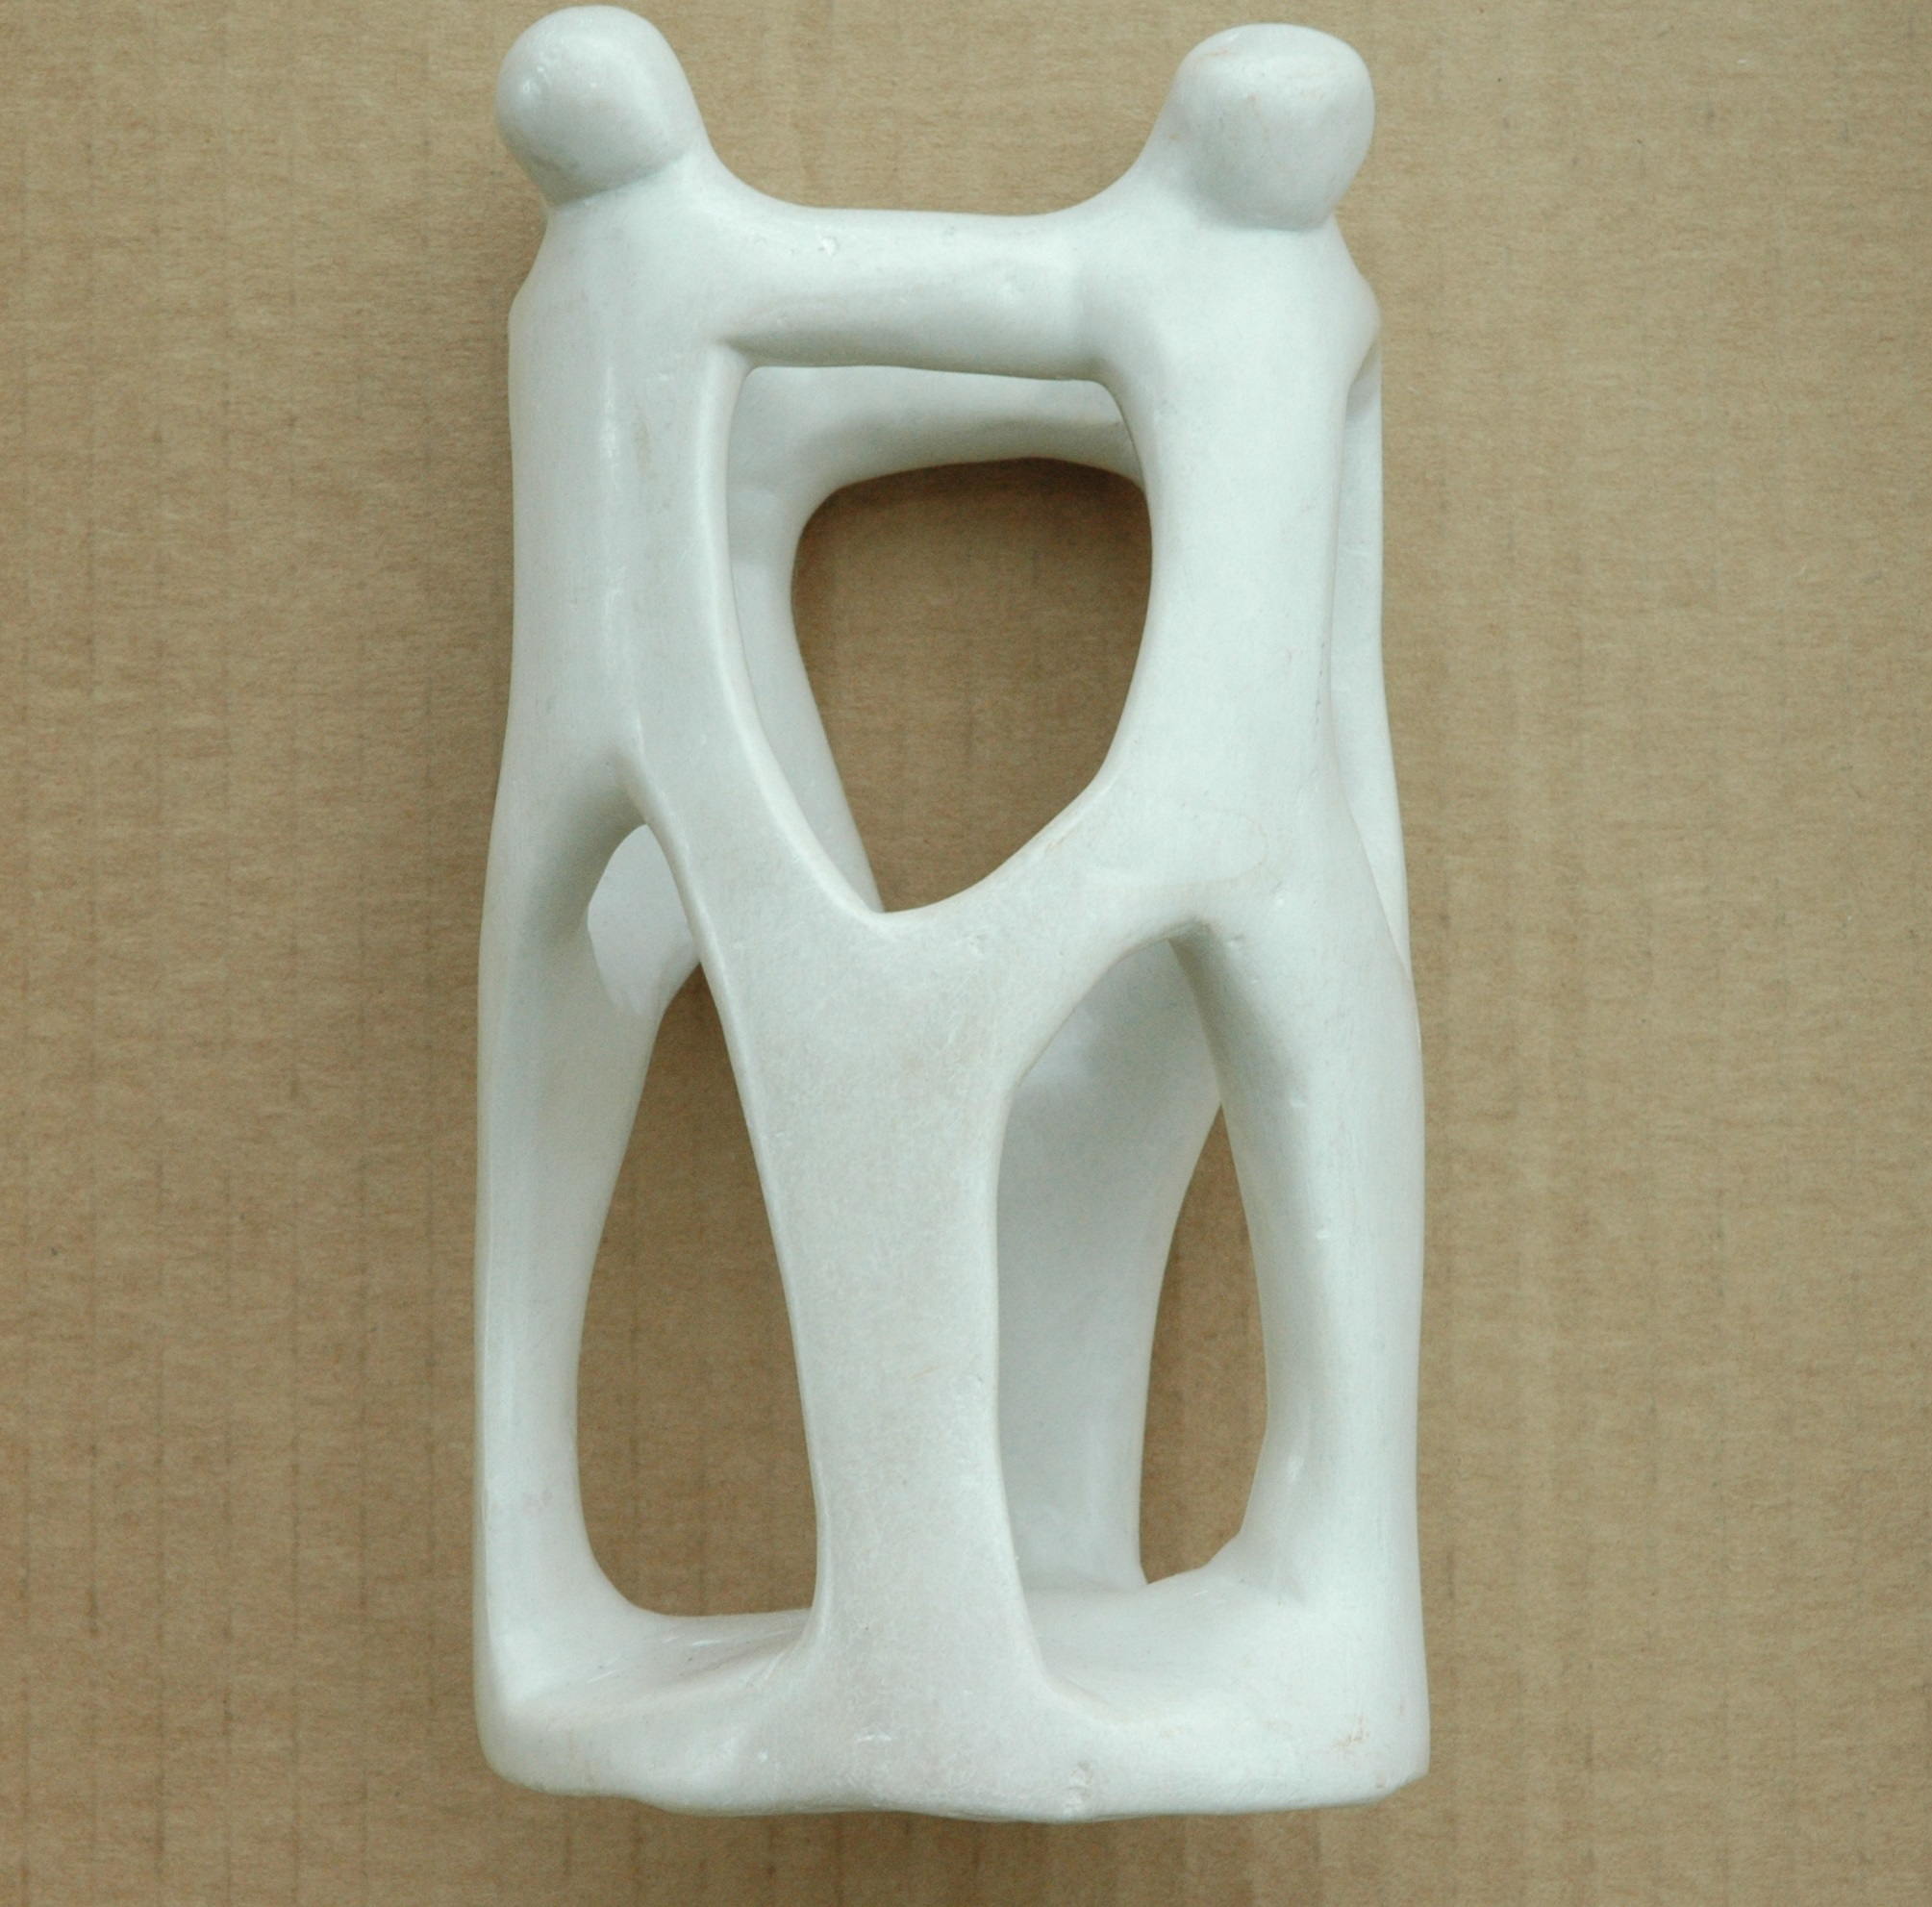
\includegraphics[width=0.33\textwidth]{interp/real_world_obj/statue/statue}} &
  \multicolumn{3}{l}{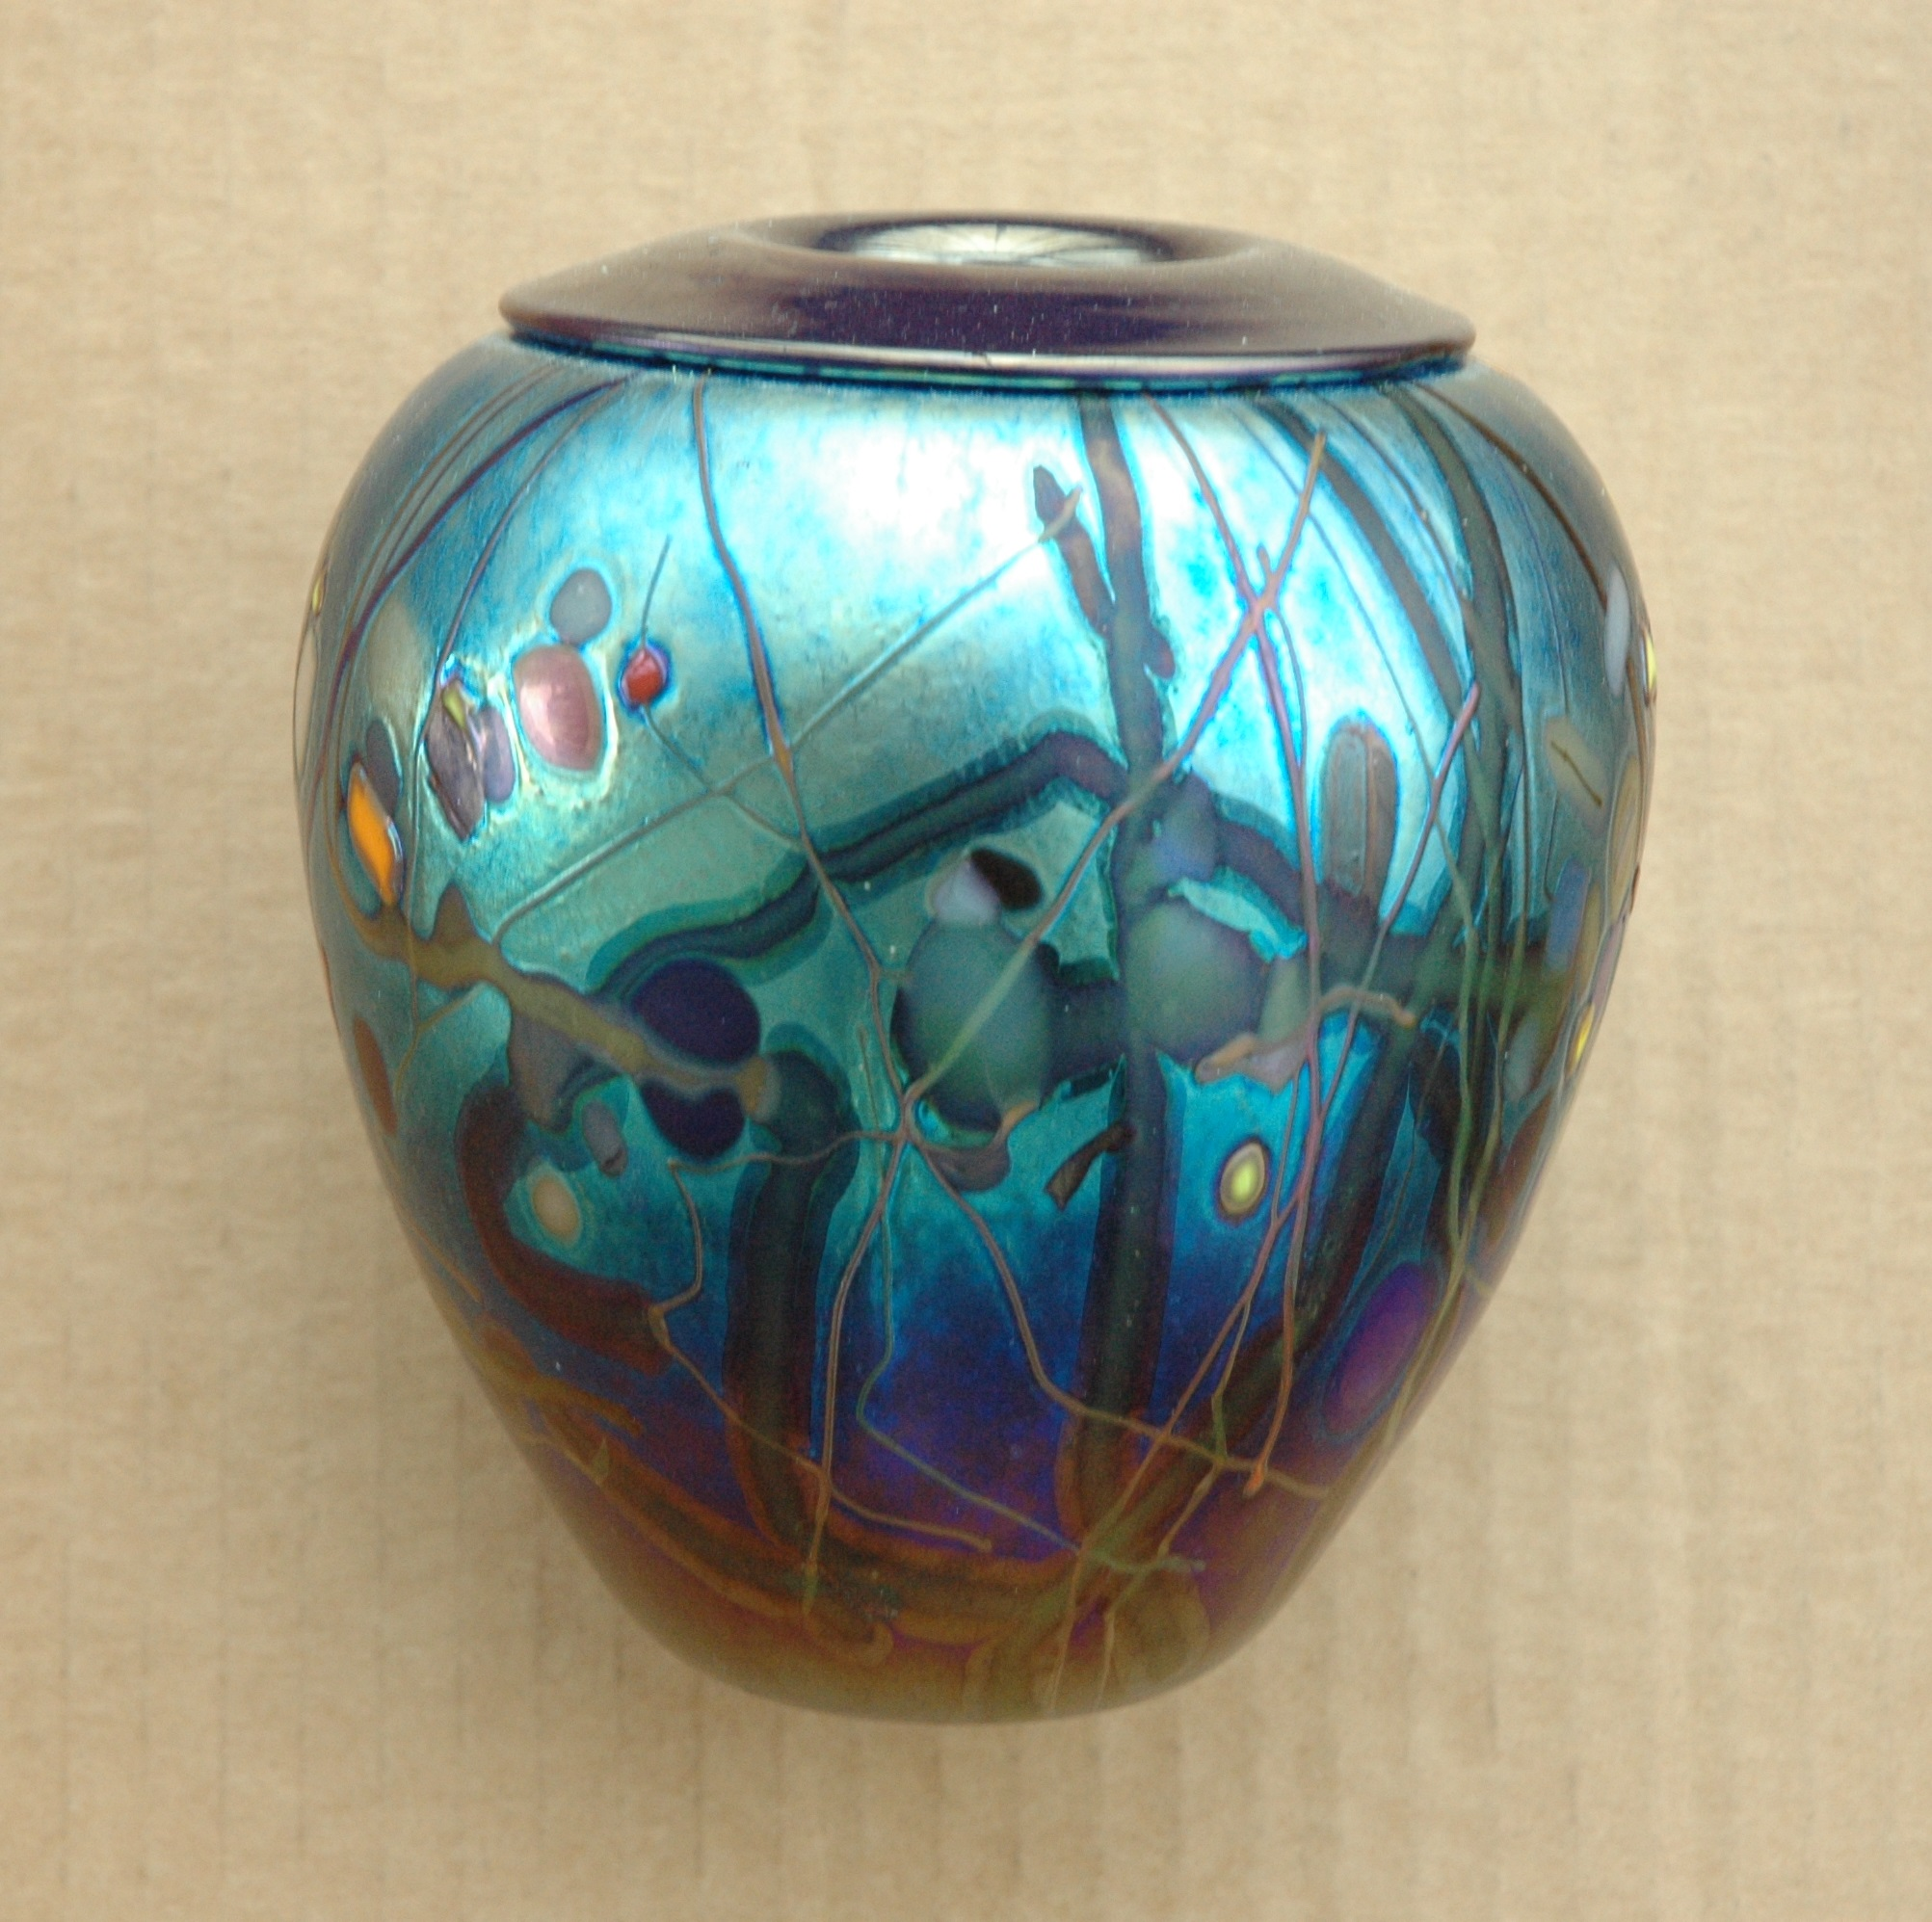
\includegraphics[width=0.33\textwidth]{interp/real_world_obj/vase/vase}}\\
  \includegraphics[width=0.1\textwidth]{interp/real_world_obj/pot/base_00} &
  \includegraphics[width=0.1\textwidth]{interp/real_world_obj/pot/base_01} & &
  \includegraphics[width=0.1\textwidth]{interp/real_world_obj/statue/base_00} & & &
  \includegraphics[width=0.1\textwidth]{interp/real_world_obj/vase/base_00} &
  \includegraphics[width=0.1\textwidth]{interp/real_world_obj/vase/base_01}\\
  \multicolumn{3}{c}{(g). pot} & \multicolumn{3}{c}{(h). statue} & \multicolumn{3}{c}{(i). vase} \\
  \end{tabular}
  \caption{Material of Real-world objects.}
  \label{fig:real_data_material}
\end{table}

\begin{table}[!htbp]
  \centering
  \begin{tabular}{l*{5}{c}}
  \hline
  \textbf{Property} & Texture & Albedo & Specular & Roughness & Best-suited Algo.\\
  \hline
  box & 0.2 & 0.8 & 0.2 & 0.2 & MVS, SL, PS\\
      & 0.5 & 0.2 & 0.2 & 0.5 & \\
      & 0.8 & 0.8 & 0.2 & 0.5 & \\
  cat0 & 0.5 & 0.5, 0.2 & 0.2 & 0.2 & None\\
  cat1 & 0.2 & 0.2 & 0.2 & 0.2 & None\\
  cup & 0.2 & 0.8 & 0.2 & 0.2 & PS, SL\\
  dino & 0.2 & 0.5, 0.8, 0.8 & 0.2 & 0.5 & SL\\
  house & 0.8 & 0.8, 0.2 & 0.2 & 0.2 & MVS\\
  pot & 0.5 & 0.2, 0.5 & 0.2 & 0.2 & MVS, SL\\
  status & 0.2 & 0.8 & 0.2 & 0.5 & PS, SL\\
  vase & 0.8 & 0.8, 0.2 & 0.2 & 0.2 & None\\
  \hline
  \end{tabular}
  \caption{Property list for the real-world objects}
  \label{tab:real_data_prop_list}
\end{table}

In Figure~\ref{fig:test_real_world_obj}, we show the reconstructions of the real-world dataset. Since we don't have the ground truth, no quantitative measures are available, only visual inspection is used. We can show that the qualitative results match the results returned by the mapping.
\begin{figure}[h!]
\centering
\begin{tabular}{lcccr}
Object & PMVS & Example-based PS & Gray SL & Best-suited Algo.\\
box &
\raisebox{-.5\height}{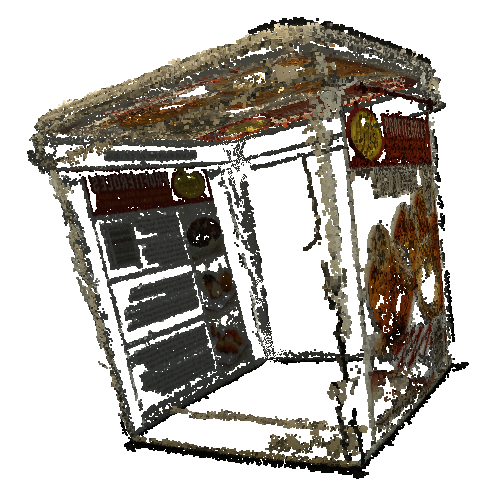
\includegraphics[width=0.2\textwidth]{interp/real_data/box/box_mvs_00}}&
\raisebox{-.5\height}{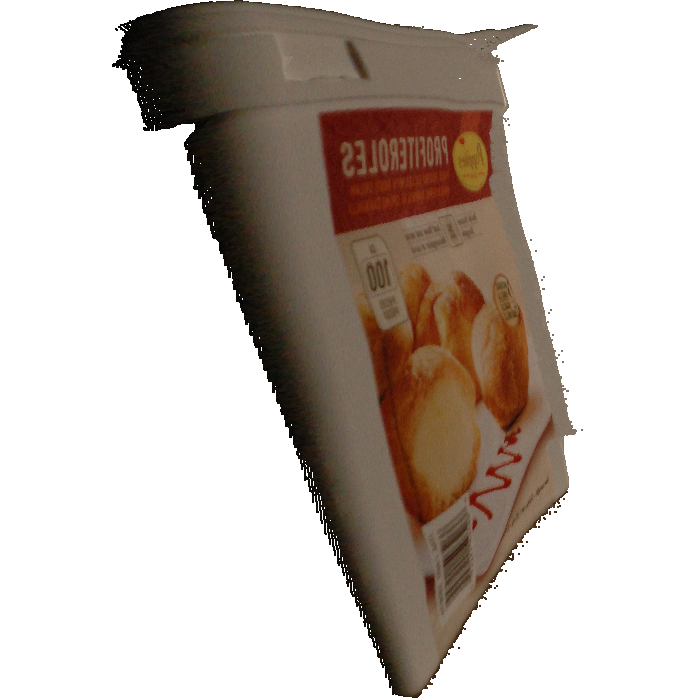
\includegraphics[width=0.2\textwidth]{interp/real_data/box/box_ps_00}}&
\raisebox{-.5\height}{\includegraphics[width=0.2\textwidth]{interp/real_data/box/box_sl_00}}&
MVS, SL, PS\\
cat0 &
\raisebox{-.5\height}{\includegraphics[width=0.2\textwidth]{interp/real_data/cat0/cat0_mvs_00}}&
\raisebox{-.5\height}{\includegraphics[width=0.2\textwidth]{interp/real_data/cat0/cat0_ps_00}}&
\raisebox{-.5\height}{\includegraphics[width=0.2\textwidth]{interp/real_data/cat0/cat0_sl_00}}&
None\\
cat1 &
\raisebox{-.5\height}{\includegraphics[width=0.2\textwidth]{interp/real_data/cat1/cat1_mvs_00}}&
\raisebox{-.5\height}{\includegraphics[width=0.2\textwidth]{interp/real_data/cat1/cat1_ps_00}}&
\raisebox{-.5\height}{\includegraphics[width=0.2\textwidth]{interp/real_data/cat1/cat1_sl_00}}&
None\\
dino &
\raisebox{-.5\height}{\includegraphics[width=0.2\textwidth]{interp/real_data/dino/dino_mvs_00}}&
\raisebox{-.5\height}{\includegraphics[width=0.2\textwidth]{interp/real_data/dino/dino_ps_00}}&
\raisebox{-.5\height}{\includegraphics[width=0.2\textwidth]{interp/real_data/dino/dino_sl_00}}&
PS, SL\\
cup &
\raisebox{-.5\height}{\includegraphics[width=0.2\textwidth]{interp/real_data/cup/cup_mvs_00}}&
\raisebox{-.5\height}{\includegraphics[width=0.2\textwidth]{interp/real_data/cup/cup_ps_00}}&
\raisebox{-.5\height}{\includegraphics[width=0.2\textwidth]{interp/real_data/cup/cup_sl_00}}&
PS, SL\\
house &
\raisebox{-.5\height}{\includegraphics[width=0.2\textwidth]{interp/real_data/house/house_mvs_00}}&
\raisebox{-.5\height}{\includegraphics[width=0.2\textwidth]{interp/real_data/house/house_ps_00}}&
\raisebox{-.5\height}{\includegraphics[width=0.2\textwidth]{interp/real_data/house/house_sl_00}}&
MVS\\
pot &
\raisebox{-.5\height}{\includegraphics[width=0.2\textwidth]{interp/real_data/pot/pot_mvs_01}}&
\raisebox{-.5\height}{\includegraphics[width=0.2\textwidth]{interp/real_data/pot/pot_ps_00}}&
\raisebox{-.5\height}{\includegraphics[width=0.2\textwidth]{interp/real_data/pot/pot_sl_00}}&
MVS, SL\\
\end{tabular}
\caption{Reconstruction results of MVS, PS, SL}
\label{fig:test_real_world_obj}
\end{figure}

\begin{figure}[h!]
\centering
\begin{tabular}{lcccr}
Object & PMVS & Example-based PS & Gray SL & Best-suited Algo.\\
statue &
\raisebox{-.5\height}{\includegraphics[width=0.2\textwidth]{interp/real_data/statue/statue_mvs_00}}&
\raisebox{-.5\height}{\includegraphics[width=0.2\textwidth]{interp/real_data/statue/statue_ps_00}}&
\raisebox{-.5\height}{\includegraphics[width=0.2\textwidth]{interp/real_data/statue/statue_sl_00}}&
PS, SL\\
vase &
\raisebox{-.5\height}{\includegraphics[width=0.2\textwidth]{interp/real_data/vase/vase_mvs_01}}&
\raisebox{-.5\height}{\includegraphics[width=0.2\textwidth]{interp/real_data/vase/vase_ps_00}}&
\raisebox{-.5\height}{\includegraphics[width=0.2\textwidth]{interp/real_data/vase/vase_sl_00}}&
MVS\\
\end{tabular}
\caption{Reconstruction results of MVS, PS, SL (cont'd)}
\label{fig:test_real_world_obj}
\end{figure}

\section{Summary}

